\documentclass[a4paper, 10pt]{article}
\usepackage{a4wide}
\usepackage[utf8]{luainputenc}
\usepackage[english]{babel}
\usepackage{parskip} % To prevent indentation of new paragraphs
\usepackage{lmodern} % Modern font with a.o. euro symbols included
\usepackage[T1]{fontenc} % Fix font encoding in the document to improve the layout
\usepackage{authblk}
\usepackage[toc,page]{appendix}
\usepackage{pdflscape}
\usepackage{environ} % For custom environments which we will probably need at some point

% Text layout packages
\usepackage{hyperref} % Hyperlinks
\usepackage{color} % For colors
\usepackage{xcolor} % For colors
\usepackage[inline]{enumitem} % For lists, possibly inline
\usepackage{fontspec} % For custom fonts
\usepackage{microtype} % For better text appearance

% Figures & References packages
\usepackage[labelfont=bf]{caption} \captionsetup{width=0.8\textwidth, font=small} % For captions
\usepackage{subcaption} % For more advanced captions, such as figure 1a, b, c
\usepackage{graphicx} % Include more types of images
\usepackage[style=numeric,citestyle=numeric-comp,natbib=true,sorting=none]{biblatex}
\addbibresource{references.bib}

% Table packages
\usepackage{booktabs} % Used for lines in tables
\usepackage{float}
\usepackage{xltabular}
\usepackage{multirow} % For row-spans besides column-spans
\usepackage{tabularx} % For tables with automatically expanding columns
\usepackage[column=C]{cellspace} \addparagraphcolumntypes{X}

%\usepackage{floatrow}
\usepackage{siunitx} \sisetup{load-configurations = abbreviations, separate-uncertainty=true, exponent-product=\cdot, output-product=\cdot} % Formatting numbers
\usepackage{listings} % For code listings
\usepackage{minted} % For code coloring (requires color)

\usepackage{csquotes}

% Fix normal tabular booktabs
\AtBeginEnvironment{tabular}{\let\xltabular\undefined}
\AtBeginEnvironment{tabularx}{\let\xltabular\undefined}

% Make italics numbers possible in siunitx columns
\robustify\itshape
\robustify\bf
\robustify\bfseries
\sisetup{detect-all=true}

% Fix link display
\hypersetup{colorlinks=false,linkbordercolor=gray!30!white,pdfborderstyle={/S/U/W 1}}

% Add Code style definitions
% Code style definitions
\definecolor{Gray}{gray}{0.95}

%\setsansfont{Segoe UI}
\newfontfamily{\cascadia}{Cascadia Mono}[NFSSFamily=Cascadia]
\renewcommand{\theFancyVerbLine}{\sffamily\textcolor[rgb]{0.5,0.5,0.5}{\scriptsize\arabic{FancyVerbLine}}}
\usemintedstyle{vs}
\renewcommand{\listingscaption}{Code sample}

\newmintinline[java]{Java}{
	mathescape,
	tabsize = 4
}

\newminted[javashort]{Java}{
	tabsize = 4,
	breaklines,
	breakautoindent = true,
	bgcolor = white,
	fontfamily = Cascadia,
	fontsize = \fontsize{8pt}{12pt}
}

\newminted[javalong]{Java}{
	linenos,
	frame = lines,
	framesep = 3mm,
	breaklines,
	breakautoindent = true,
	fontsize = \fontsize{8pt}{10.5pt},
	tabsize = 4,
	bgcolor = white,
	mathescape = true,
	texcomments = true
}

\newminted[cpplong]{C++}{
	linenos,
	frame = lines,
	framesep = 3mm,
	breaklines,
	breakautoindent = true,
	fontsize = \fontsize{8pt}{10.5pt},
	tabsize = 4,
	bgcolor = white,
	mathescape = true,
	texcomments = true
}

\newminted[kotlinlong]{Kotlin}{
	linenos,
	frame = lines,
	framesep = 3mm,
	breaklines,
	breakautoindent = true,
	fontsize = \fontsize{8pt}{10.5pt},
	tabsize = 4,
	bgcolor = white,
	mathescape = true,
	texcomments = true
}

% Define some macros
\makeatletter
\newcommand{\source}{\@ifstar\@@source\@source}
\newcommand{\@source}[2]{\textsc{Source:} {\it ``#1''} #2}
\newcommand{\@@source}[1]{\textsc{Source:} #1}
\makeatother


\begin{document}

\begin{titlepage}
\addtolength{\hoffset}{0cm}
	\centering
	
\includegraphics[width=\textwidth]{images/rug_logo.jpg}
	\par\vspace{0.5cm}
    \textbf{Faculty of Science and Engineering - University of Groningen}\\
    % \textbf{Department of Computing Science}\\
    \vspace{1cm}
	{\scshape\LARGE Software Maintenance \& Evolution \par}
	\vspace{0.5cm}
	
	\noindent\makebox[\textwidth]{\rule{\textwidth}{0.4pt}}
 	{\huge\bfseries Design Patterns in \textsc{Apache MINA}  \par }

	\noindent\makebox[\textwidth]{\rule{\textwidth}{0.4pt}}
	 	{\large\bfseries Exploring the rationale of introducing and removing design patterns in \textsc{Apache MINA}  \par}
	 	
    \vspace{0.5cm}
    
\includegraphics[width=0.3\textwidth]{images/mina_logo.png}
	\par\vspace{0.5cm}	 	
	 
	
% 	\vspace{1.5cm}
	
	{\itshape Authors:}  \par
	 
	 Alina \textsc{Matei} 
	\vspace{0.1cm}\\
	  Floris \textsc{Westerman} 

		
    \vspace{1cm}
	{\itshape Coordinator:} \par
	Dr. Mohamed \textsc{Soliman}
	\vspace{0.5cm}\\
	{\itshape Teaching assistant:} \par
	Filipe \textsc{Capela}
	
	
    \vfill

% Bottom of the page
	{\large \today\par}
\end{titlepage}
\newpage
\tableofcontents
\newpage
\listoffigures
\newpage

\section{Introduction}
\label{sec:introduction}

For the purpose of this report, we focus on analysing the Open Source application framework entitled Apache MINA. Apache MINA (Multipurpose Infrastructure for Network Applications) \cite{mina-website} is a network application framework written in Java. Its main selling point is that it facilitates the creation of high performance and scalable network applications. The core element of MINA is the abstract, event-driven, asynchronus API it provides which facilitates the implementation of several transport protocol suites such as TCP/IP or UDP/IP via Java NIO \cite{oracle-nio}. Therefore, MINA is often referred to as a NIO framework library, networking socket library or client server framework library.

\subsection{Community and background}
Apache MINA was created in 2004 through the joint effort and ideas of Trustin Lee and Alex Karasulu, based on its predecessor Netty2\footnote{Currently Netty exists as an independent Java client-server framework \cite{netty}.}. According to the GitHub repository of the MINA project \cite{mina-github}, there are 18 active contributors; the project sums up a total of 46,461 lines of code. There are a total of 60 official releases, the latest stable ones being 2.0.21 and 2.1.3. For the purpose of this report, we will focus mainly on version 2.1.3. Apart from GitHub, the MINA community uses Jira issue tracking \cite{mina-jira} and mailing lists for both users (i.e. users-subscribe@mina.apache.org) and developers (i.e. dev-subscribe@mina.apache.org). 

\subsection{Goals of the report}
%% this needs to be updated as we extend the document
The core motivation of this report is to analyse the rationale behind using design patterns in an Open Source project such as Apache MINA. Our main focus is to identify design patterns (or the lack there of) in the codebase and research the motivation of the developers for introducing or removing the corresponding patterns.

The first steps undertaken for this purpose are to identify the core requirements of MINA (see section \ref{sec:analysis_requirements}) and understand the Open Source document from an architectural stand point (see section \ref{sec:analysis_components}). Next, the design patterns are being recovered using the appropriate tools described in section \ref{sec:pacito_dev}. The analysis of the recovered patterns is conducted in section \ref{sec:pattern_analysis} from both a quantitative and qualitative perspectives. Finally, conclusions and future work are presented in sections \ref{sec:conclusion} and \ref{sec:futurework}, respectively.

\subsection{Project's GitHub}
All the materials supporting the claims made in this report can be found at \url{https://github.com/FWest98/SME}.

\newpage
\section{System Analysis: architecturally significant requirements}
\label{sec:analysis_requirements}

In the section at hand, we report the findings of the top-down analysis of the Apache MINA framework. We perform a thorough investigation of various sources, as described in section \ref{sec:overview_of_sources}, without considering the codebase of the project, in order to distil the core functionalities of the MINA (see section \ref{sec:features}) and the significant quality attributes (see section \ref{sec:quality_attributes}), which are key drivers for the architecture of the project.

\subsection{Overview of sources}
\label{sec:overview_of_sources}
For the top-down analysis, we use the following sources:
\begin{enumerate}
    \item Official website \cite{mina-website}
    \item Documentation \cite{mina-docs}
    \begin{enumerate}
        \item Presentations \cite{mina-talk2006, mina-talk2008}
        \item User guide \cite{mina-userguide}
        \item Tutorials (Quick Start guide) \cite{mina-qsguide}
    \end{enumerate}
    \item API documentation \cite{mina-reference} \footnote{This will mostly be of help for determining the architectural components}
    \item User testimonials \cite{mina-testimonials}
\end{enumerate}
The User guide includes various tutorials that will aid us in understanding the full extent of the project's functionalities. The User testimonials are an informal source, however we believe it will strengthen the validation of the quality attributes.

The information significant for the understanding of the requirements of the project is annotated and presented in this section to support and validate our analysis. We present excerpts from the sources with their corresponding links that can be easily checked.

\subsection{System's features}
\label{sec:features}
Researching the official documentation, the features offered by MINA immediately become apparent. An overview of the features is presented in figure \ref{fig:features}, as extracted from the documentation \cite{mina-docs}. Most of these features correspond to the functional requirements of the framework. We identify the following 2 core architecturally significant functional requirements, as distilled from these features and complementary sources:
\begin{itemize}
    \item Provide a layer of abstraction on top of the networking layer, which hides the differences between Blocking and Non-blocking IO, which simulates a blocking mode. This enables the development of network applications which, in essence, consist of a server and a client side communicating over some network protocol (e.g. TCP, UDP). 
    
    \source{[...] the best solution is to hide this aspect by writing a framework that mimics a blocking mode. This is what MINA does!}{\cite[Sec. 1.2]{mina-userguide}}
    
    \item Standardize the IO application vision w.r.t. transport types (e.g. TCP/IP, UDP/IP, serial and in-VM pipe  communication, custom).
    
    \source{It provides a common IO vision to an application that needs to communicate over TCP, UDP or whatever mechanism. [...] MINA does not only handle TCP and UDP, it also offers a layer on top of serial communication (RSC232), over VmpPipe or APR.}{\cite[Sec. 1.2]{mina-userguide}}
\end{itemize}

\begin{figure}
    \centering
    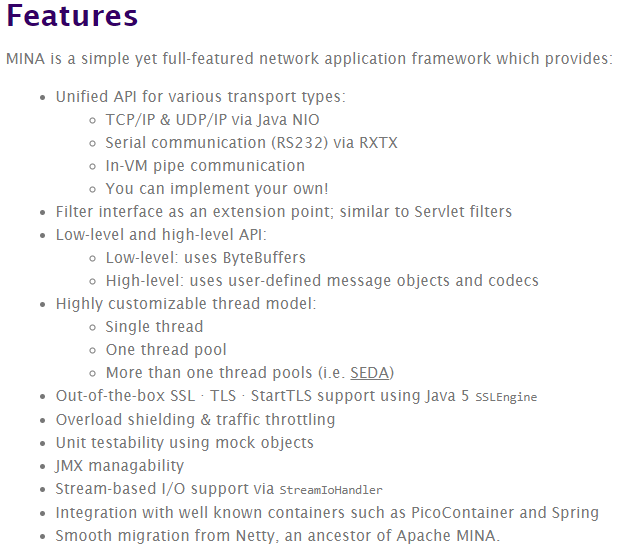
\includegraphics[width=0.7\textwidth]{images/features.png}
    \caption{An overview of the features provided by Apache MINA extracted from the official documentation.}
    \label{fig:features}
\end{figure}

The core feature of the framework is, therefore, the \textit{Unified API for various transport types}. The remaining features mentioned in figure \ref{fig:features} are additions to the core MINA project that not only extend the functionality of the framework, but, most importantly, ensure the expected quality attributes discussed below.

\subsection{Quality attributes}
\label{sec:quality_attributes}

\source{Apache MINA is a network application framework which helps users develop high performance and high scalability network applications easily.}{\cite{mina-website}}

From this definition of Apache MINA on the official website it follows that the key drivers of the project are \textit{performance} and \textit{scalability}. We have further identified other significant quality attributes of the framework itself, as well as the MINA based applications, which are individually explored below and correlated to the features or functionalities through which these qualities are achieved.

\subsubsection{Performance \& scalability}
MINA has been specifically designed to work both on the client and server side, performance and scalability therefore being of paramount importance for adapting to server requirements. In terms of design decisions, NIO communication has been chosen as the building block of MINA since it offers better scalability for a large number of connections (i.e. over a few thousands). The performance of the framework has been tested over AMQP (Advanced Message Queuing Protocol), the results are showcased in the introductory presentation \cite{mina-talk2006}. As an example, MINA offers \textit{overload shielding \& traffic throttling} to ensure these qualities.

\source{Writing a server makes it critical to have a scalable system, which is tunable to fit the server needs, in terms of performance and memory usage. This is what MINA is good for, making it easy to develop you server.}{\cite[Sec. 1.2]{mina-userguide}}

\source{This is true for up to a few thousands of connected users, but up to a point, the BIO approach just stops scaling; you won’t be able to handle millions of connected users using one thread per user! NIO can. Now, one other aspect is that the time spent in the MINA part of your code is probably non significant, ...}{\cite[Sec. 1.2]{mina-userguide}}


\subsubsection{Usability}
Programming network application has a stigma of being regarded as low level programming and a highly complicated task. MINA comes as a response and provides a user friendly framework. This is achieved through the various features which allow for high degrees of user customization: own implementation of transport types, high-level API with user defined message objects, customizable thread model (see figure \ref{fig:features}). Moreover, the extensive documentation sources (user guide, tutorials etc.) aid the user in the implementation of their own applications on top of MINA.

\source{Ease of use When you have no special performance requirements, MINA is probably a good choice as it allows you to develop a server or a client easily [...] You could probably write your server with only a few lines of code...}{\cite[Sec. 1.2]{mina-userguide}}

\source{You just have to design your application on top of MINA without having to handle all the complexity of the newtork layer.}{\cite[Sec. 2.1]{mina-userguide}}

\source{This gives you the ease of mind that you won’t have to spend hours on some cryptic errors in your own implementation of the network layer.}{\cite[Sec. 1.2]{mina-userguide}}

\source*{Figure \ref{fig:usability_extensibility} shows the ease of use of the framework in creating network applications (i.e. a simple echo server).}


\subsubsection{Testability}
The unified API offered by MINA follows an abstract design approach; this supports unit tests. As seen in figure \ref{fig:features}, the framework is unit test friendly and also provides mock objects to increase the testability of the applications developed on top of MINA.

\source{Unit-testable, abstract API, out-of-the-box mock objects}{\cite[p.6]{mina-talk2008}}

\subsubsection{Extensibility}
%run time extensible through filters
Applications built on top of MINA can be easily extended. This is implemented through the filters feature (see figure \ref{fig:features}). The filters can modify the application behaviour at runtime (e.g. logging filter, blacklist remote address filter); the filters are dynamically activated which provides additional flexibility for the MINA based applications. Figure \ref{fig:filters} shows an overview of the out-of-the-box filters included in the framework. As an advanced topic, users can configure their own IO filters, which reinstates the high customization degree of the framework.

\source{Extensible, Runtime modification of application behavior using `filters'.}{\cite[p.7]{mina-talk2008}}

\source{Many out-of-the-box filters are provided to accelerate network application development pace by simplifying typical cross-cutting concerns using the out-of-the-box filters.}{\cite[Sec. 5]{mina-userguide}}

\source*{Figure \ref{fig:usability_extensibility} presents options for extending the functionality of a simple server application.}

\subsubsection{Maintainability \& reusability}
MINA has been designed with the maintainability and reusability concerns in mind; this is immediately apparent when considering the high-level architecture of the framework. A high-level overview is presented in figure \ref{fig:architecture}. A more in depth account of the architectural components is presented in section \ref{sec:analysis_components}. For now, we foucs on the layered structure which enforces separation of concerns: the business logic is completely separated from the processing of the IO. Moreover, at the IO Service and Filter Chain levels, out-of-the-box components are provided, allowing the user to focus mainly on the application layer which involves the logic of handling the messages. The separation of concerns involved with the architecture design, together with the variety of pre-made components, enforce the maintainability and reusability of MINA.

\source{Broadly, MINA based applications are divided into 3 layers: \begin{itemize*}\item I/O Service - Performs actual I/O \item I/O Filter Chain - Filters/Transforms bytes into desired Data Structures and vice-versa \item I/O Handler - Here resides the actual business logic \end{itemize*}}{\cite[Sec. 2.1]{mina-userguide}}

\source*{Figure \ref{fig:reusability} showcases the modular and reusable nature of components which build the MINA architecture.}

\begin{figure}
    \centering
    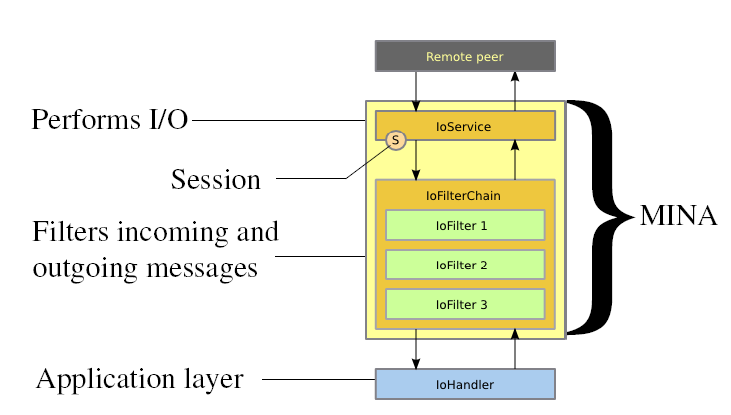
\includegraphics[width=\textwidth]{images/architectural_overview.png}
    \caption{MINA architectural overview as presented in the presentation "MINA in Real Life (ApacheCon EU 2009)".}
    \label{fig:architecture}
\end{figure}




\subsubsection{Stability}
MINA is a proven system with a stable architecture; it is presently used by various applications, therefore a drastic structural change is unlikely. None the less, MINA has had a stable evolution empowered by the component modularity of its architecture: the core of the architecture remained stable, while components have been added to extend the functionality of the framework (e.g. the filters functionality mentioned above). The sustained effort of maintaining the framework and its documentation (especially the API design) also contributes to its stability.

\source{A proven system MINA is used by many applications all over the world. There are some Apache projects based on MINA, and they are working pretty well.}{\cite[Sec. 1.2]{mina-userguide}}

\subsubsection{Integration \& manageability}
MINA offers integration with a number of third-part systems (e.g. PicoContainer, Spring) among which JMX (Java Management Extensions, see figure \ref{fig:features}). Through connection with the JMX API, the management of MINA based applications is facilitated.

\source{Java Management Extensions (JMX) is used for managing and monitoring java applications. This tutorial will provide you with an example as to how you can JMX-enable your MINA based application.}{\cite[Sec. 16]{mina-userguide}}

\source*{Figure \ref{fig:manageability} presents the added management functionality provided through the JMX integration.}
\subsection{Quality attributes validation}
Quality attributes pertain to non-functional requirements of a system. They can span the entire system and are difficult to quantify. Since non-functional qualities of a system are closely related to the user's needs and expectations of the system, we present a series of user informal evaluations of MINA in order to validate its quality attributes; these evaluations are extracted from \cite{mina-testimonials}.

\begin{itemize}
    \item \textsc{Performance, Scalability, Maintainability}: \textit{``I found that Apache MINA really did fulfill its promise and implementing a high-performance, scalable and extensible network server was easy using it. MINA also helps very cleanly separate network communication and application level message processing logic.''} 
    \item \textsc{Performance, Stability, Usability}: \textit{``We found the speed and stability of MINA to be excellent. And although we are still using MINA 0.8.1, we found the API very elegant and easy.''}
    \item \textsc{Performance, Stability, Testability}: \textit{``[...]MINA was a real treat as it saved a lot of time, is well written and gets more testing than our in house QA would be able to cover. The speed and stability of our app on top of MINA has been excellent.''}
    \item \textsc{Usability}: \textit{``[...]It makes writing server applications simple and is much easier to use than Java’s NIO libraries. Because of MINA’s stability and ease of use, we plan on using MINA more in our future projects.''}
\end{itemize}
\newpage
\section{System Analysis: architectural components}
\label{sec:analysis_components}
In this section, we present our investigation into the architecture of the MINA framework. The main focus is to comprehend the structure of the architecture, the dependencies between components and their responsibilities. 
\subsection{Analysis steps}
For conducting this analysis, we investigate the source code \cite{mina-github}, the API documentation \cite{mina-reference} and use the Structure101 tool \cite{structure101} to obtain a clear view of the architecture.\\\\
The first step is importing the MINA project intro Structure101. For clarity and aiding reproducibility, we specify the steps:
\begin{enumerate}
    \item Download latest stable version of MINA, for this report we use version 2.1.3.
    \item Install MINA using command \texttt{MVN CLEAN INSTALL -DSKIPTESTS}
    \item Import MINA as a Maven project in Structure101 through the root pom file.
\end{enumerate}
Having the Structure101 project, we analyze the architecture at a high-level of abstraction; we show how the packages interact and if any patterns are captured by the high-level architecture. This information is presented in section \ref{sec:archi_overview}.\\\\
Following the general overview, each package is individually analysed in section \ref{sec:component_analysis}. For this analysis, we consider the following aspects:
\begin{itemize}
    \item Initial structure of the package
    \item If necessary (i.e. tangles are present), our restructuring of the package
    \item Dependencies and dependents
    \item Inner dependencies
    \item Components and responsibility
    \item Identified patterns
    
\end{itemize}
Finally, we consider one use case of MINA and analyse it from an architectural point of view: how do the architecturally components interact with each other in order to fulfill the functionality of the use case? The use case presents the construction of a MINA server. We will also present the corresponding JAVA implementation.


\subsection{High-level overview of the architecture}
\label{sec:archi_overview}
An account of the high-level architecture structure is presented in figure \ref{fig:packages_structure}; we identify 9 main structural modules:
\begin{enumerate}
    \item \texttt{mina-integration-jmx}: supports JMX integration for managing and monitoring MINA applications.
    \item \texttt{mina-integration-xbean}
    \item \texttt{mina-integration-ognl}
    \item \texttt{mina-integration-beans}
    \item \texttt{mina-filter-compression}: the implementation of a \texttt{IOFilter} which compresses all data using \texttt{JZlib}\cite{jzlib}.
    \item \texttt{mina-http}: implementation of \texttt{http} communication using MINA; exposes an API for MINA applications using the \texttt{http} protocol.
    \item \texttt{mina-statemachine}: offers support for complex applications that would like to implement object state-based behaviour; \texttt{mina-statemachine} implements a improved reinterpretation of the State pattern \cite{state_pattern}.
    \item \texttt{mina-transport-apr}: provides support for APR (Apache Portable Runtime)\cite{apr} transport.
    \item \texttt{mina-core}: the core implementation of the MINA framework; offers the basic functionality by exposing an API for the MINA based applications.
    
\end{enumerate}

\begin{figure}[H]
    \centering
    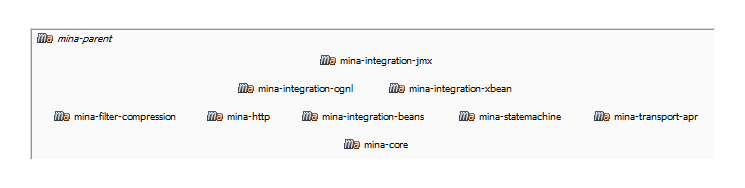
\includegraphics[width=\textwidth]{images/MINA_packages_overview.png}
    \caption{Overview of the package structure of the MINA framework.}
    \label{fig:packages_structure}
\end{figure}

Figure \ref{fig:overview_package_dependencies} in the Appendix shows the overall dependencies between the high-level architectural modules. It is clear that the \texttt{mina-core} module is the back-bone of the framework, the rest of the packages directly or indirectly being dependent on this module (i.e. dependencies flow from top to bottom). Another noticeable aspect is the dependencies between the integration packages, therefore we propose the following restructuring shown in figure \ref{fig:packages_restructure}.

\begin{figure}[H]
    \centering
    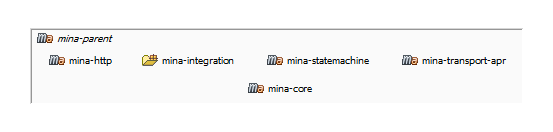
\includegraphics[width=\textwidth]{images/MINA_overview_restructured.png}
    \caption{Overview of the restructured packages of the MINA framework.}
    \label{fig:packages_restructure}
\end{figure}

After the proposed restructuring, the responsibilities of the main modules can be traced as follows, presented in order of importance:
\begin{enumerate}
    \item Implementation of API exposing core functionality of the MINA framework: \texttt{mina-core}
    \item Performance optimization: \texttt{mina-transport-apr}
    \item Additional or advanced functionality which extends the core:  \texttt{mina-http}, \texttt{mina-statemachine}
    \item Third-party integration: \texttt{mina-integration}
\end{enumerate}
In this report, we will emphasize the investigation of the core architecture, in other words, we will focus predominantly on the \texttt{mina-core} module. We expect this module to follow the architectural schema presented in figure \ref{fig:architecture}, since it captures the underlying structure of MINA based applications. This entails that the core module implements the transport layer (i.e. connection to the remote peer as presented in figure \ref{fig:architecture}), the IO service layer, the filters (i.e. IOFilterChain layer in \ref{fig:architecture})  which process the IO and the business logic layer (i.e. IOHandler in figure  \ref{fig:architecture}, a this level the user is able to implement their own logic), all of these components being presided by a session. Keeping in mind the goal of the report at hand, we can already guess the usage of the Layers pattern \cite{archi_patterns}. \\\\
Other remarks regarding the high-level architecture related to the proposed restructuring. Our decision of clustering the integration packages is based on the top-down dependencies between the integration packages as shown in figure \ref{fig:dependencies_integration} in the Appendix, as well as on their serving a common purpose: integration with a third-party entity. The \texttt{mina-filter-compression} has been moved to the core module and grouped together with the useful filter implementations provided by MINA. For the case of the remaining modules that provide additional functionality, we decided to keep the structure proposed by the MINA development team since they serve different purposes and they create more dependencies if included in the core. Their only commonality is that they have been added to extend or optimize the core functionality. Their addition is also fairly new, they have been introduced in version 2.0 (for reference, we analyze Mina version 2.1.3).

\subsection{Component analysis}
\label{sec:component_analysis}
\subsubsection{MINA core}
\textsc{Initial structure}: Appendix, figures \ref{fig:mina_core_initial}, \ref{fig:mina_core_initial_detailed}, \ref{fig:mina_core_core_initial}.  \\
\textsc{Issues and restructuring}: In the initial dependency diagram (i.e. figure \ref{fig:mina_core_dependencies_initial} in the Appendix), cyclic dependencies are marked in red. With the restructuring, we attempted to overcome this problem. However, the nature of the code did not allow for this dependencies to be eliminated. We have, nonetheless, isolated the tangles and reduced the `tangle percentage' from 75\% to 45\%. Diagrams after restructuring are presented in the Appendix, figures \ref{fig:mina_core_restructured}, \ref{fig:mina_core_core_restructured}.\\
\textsc{Dependencies}: None \\
\textsc{Dependents}: All the other modules\\
\textsc{Inner dependencies}: Appendix, figure \ref{fig:mina_core_dependencies_restructured} shows inner dependencies after restructuring.\\
\textsc{Overall responsibility and scope}: This module represents the back-bone of the framework; it spans the base elements that provide support for creating applications using MINA; all other extensions in functionality, integrations or optimizations are highly reliant on this core. Apart from supporting the basic implementation of MINA based client-server applications, it provides useful implementations of IO processing filters, IO handlers and support for the development of MINA based proxy servers.\\
\textsc{Components}: the components are listed as presented in after the restructuring of the architecture:
\begin{enumerate}
    \item \texttt{mina-core-core}: main component of the module, follows the architecture presented in figure \ref{fig:architecture}; it comprises of the crucial components which provide the core functionality of the MINA framework, each components is described in detail in terms of their responsibilities.
        \begin{enumerate}
            \item \texttt{mina-core-core-service}: the most important part of the MINA architecture, it provides crucial IO services and manages the communication sessions with the remote peers. The main responsibilities are managing communication  (i.e. transmits data both ways reads \& writes), listening for \texttt{IOEvent}s, managing \texttt{IOSession}s (creation and deletion, detecting idleness), invoking the \texttt{IOHandler} upon certain events (e.g. messaged received), managing filter chain creation. The \texttt{IOService} interface is implemented by two core classes which provide the desired client-server implementation supported by the framework: \texttt{IOAcceptor}, the server side, and \texttt{IOConnector}, the client side. An overview of all the responsibilities of this module is shown in figure \ref{fig:service_responisbilities}, in the Appendix.
            \item \texttt{mina-core-core-session}: an \texttt{IOSession} represents a client-server connection (i.e. whenever a client connection is established, a new session is created); a session has a \texttt{IOSessionConfig} (e.g. sending/receiving buffer size, idle time etc.) and some user set \texttt{IOSessionAttribute}s (i.e. user defined data that must be persist during the session life-time, this is store in a dedicated \texttt{IOSessionDataStruct} for each session). The \texttt{SessionState} represents the state of the session (see figure \ref{fig:session_lifecycle} in the Appendix). Each session is correlated with a filter chain, all in-going or out-going data is processed  by the chain; moreover, the session is associated with an \textt{IOHandler} which is the communication point with the actual application (it implements the business logic based on the messages/events received). The handler will dispatch the messages received from the session, as well as responding by requesting writes in return. The session handles read/write requests via the \texttt{IOProcessor} which performs the actual IO.
            \item \texttt{mina-core-core-IOEvent}: defines an \texttt{IOEvent}, their types and filter events.
            \item \texttt{mina-core-core-IOFilter}: basic implementation of the \texttt{IOFilter} and \texttt{IOFilterChains}; using the \textit{Adapter} pattern, supports the creation of individual filters or chained filters using a customizable chain filter builder; a filter chain filters all IO events and requests between \texttt{IOService} and \texttt{IOHandler}.
        \end{enumerate}
    \item \texttt{mina-core-proxy}: while \textt{mina-core-core} provides the resources for implementing client-server applications, it provides the support for writing a MINA based proxy server; the proxy module follows the same architecture, providing specific proxy functionality for handlers, filters and sessions which complement the core \textt{IOService}.
    \item \texttt{mina-core-transport}: offers support for several transport types for MINA based applications
        \begin{enumerate}
            \item \texttt{mina-core-transport-socket}: TCP \& UDP implement based on NIO Java API, extended with support for active polling strategies (e.g. NIO select call strategy)
            \item \texttt{mina-core-transport-vmpipe}: in-VM pipe communication (removes overhead of encoding/decoding transmitted data when communication occurs within the same virtual machine).
        \end{enumerate} 
    \item \texttt{mina-core-handler}: useful implementations for \texttt{IOHandler}s
        \begin{enumerate}
            \item \texttt{mina-core-handler-chain}: offers support for implementing sequentially layered protocols via the \textit{Chain of Responsibility pattern}.
            \item \texttt{mina-core-handler-demux}: supports implementation of complex protocols by handling the received data by multiple sub-handlers.
            \item \texttt{mina-core-handler-stream}: a handler adapted for data streams.
            \item \texttt{mina-core-handler-multiton}: enables the creation of one handler per session (as opposed to a handler managing multiple session) via the \textit{Multiton pattern}.
        \end{enumerate}
    \item \texttt{mina-core-IOFilterType}: various useful IOFilter implementations (e.g. logging filter which logs all session communication events, for example "idle session", "messaged received" etc; keep alive filter which offers the ability to keep the connection alive even if data is not being transmitted)
        \begin{enumerate}
            \item \texttt{mina-core-IOFilterTypes-codec}: filter implementations which offer support for protocol development using the codec concept (i.e. a pair of coder/decoder for encoding/decoding specific types of data). 
        \end{enumerate}
    \item \texttt{mina-core-util}: miscellaneous classes used by the entire module, including a custom buffer implementation which replaces the NIO ByteBuffer.
\end{enumerate}
\textsc{Identified patterns}: Chain of Responsibility, Multiton, Adapter, Codec concept.

\subsubsection{MINA integration}
\textsc{Initial structure}: Appendix, figures \ref{fig:jmx_integration}, \ref{fig:ognl_integration}, \ref{fig:xbean_integration}, \ref{fig:beans_integration} \\
\textsc{Issues and restructuring}: No cyclic dependencies\\
\textsc{Dependencies}: \texttt{mina-core}\\
\textsc{Dependents}: None\\
\textsc{Inner dependencies}: Appendix, figure \ref{fig:dependencies_integration}\\
\textsc{Overall responsibility and scope}: Integration with JMX for application management which is built on top of JavaBeans and OGNL integration.\\
\textsc{Components}:
\begin{enumerate}
    \item \texttt{mina-integration-beans}: supports integration of JavaBeans; it implements the \texttt{PropertyEditor} class in order to create convertor classes which transform string objects into various other predefined Java classes (e.g. strings to sets, strings to patterns, strings to files).
    \item \texttt{mina-integration-ognl}: supports integration with the OGNL (Object-Graph Navigation Language) for tasks like finding \texttt{IOSession}s that match a certain OGNL expression or defining OGNL property accessors for IO filters, services and sessions.
    \item \texttt{mine-integration-xbean}: miscellaneous classes mainly adapting the JavaBeans integration with the rest of MINA. 
    \item \texttt{mina-integration-jmx}: supports integration with JMX (Java Management Extensions); it offers the possibility to manage \texttt{IOService}s and \textt{IOSession}s. As per figure \ref{fig:dependencies_integration} in the Appendix, the JMX integration it relies on the achieved integrations described above.
\end{enumerate}\\
\textsc{Identified patterns}: None, possibly a Factory pattern.

\subsubsection{MINA state machine}
\textsc{Initial structure}: Appendix, figures \ref{fig:statemachine_initial}, \ref{fig:statemachine_initial_dependencies}.\\
\textsc{Issues and restructuring}: Cyclic dependencies between the state and transition; for the restructuring, we only reorganized the package, however we could not compensate for the dependency; see Appendix, figures \ref{fig:statemachine_restructured}. \\
\textsc{Dependencies}: \texttt{mina-core}\\
\textsc{Dependents}: None\\
\textsc{Inner dependencies}: Appendix, figure \ref{fig:statemachine_restructured_dependencies} shows inner dependencies after restructuring. \\
\textsc{Overall responsibility and scope}: Extends the core functionality of MINA by supporting the implementation of state based applications; MINA \texttt{statemachine} is similar to the \textit{State} pattern and aims at tackling complexity by organizing the application's process flow into states and transitions. An example is presented in the Appendix, figure \ref{fig:statemachine_example}. We will use this example further on to explain the components of this package. \\
\textsc{Components}: 
\begin{enumerate}
    \item \texttt{State}: a class that implements the state which corresponds with the ellipses (i.e. 'playing', 'pausing') in figure \ref{fig:statemachine_example} in the Appendix. 
    \item \texttt{transition}: implements the transition between \texttt{State}s; a \texttt{Transition} reacts or accepts an \texttt{Event}; upon processing the event, a \texttt{MethodTransition} is executed, which leads to the next \texttt{State} corresponding to the \texttt{Transition}; sometimes no method is required and the transition then just changes the state (goes to next state).
    \item \texttt{event}: \texttt{Event}s trigger \texttt{Transition}s and correspond to methods to be invoked over the transition. Some examples of events that are related to state changes are IO filter and handler events.
    \item \texttt{annotation}: a \texttt{Transition} requires 3 fields: \texttt{inState}, \texttt{method}, \texttt{nextState}; the \texttt{annotation} module defines several interfaces that create the 'annotation' of various types of transitions; these 'annotations' must be defined as the 'rules' of the state machine and capture all the methods in the machine and when these methods can be invoked (i.e. between which states).
    \item \texttt{StateMachine}: based on the \texttt{Transition} annotations defined (i.e. the 'rules'), a \texttt{StateMachine} object is created using the \textit{Factory} pattern. The \texttt{StateMachine} can be seen as a collection of 'rules', however it has no knowledge of the implementation of the transition methods. For this purpose, a \texttt{StateMachineProxyBuilder} is used; this correlates the 'rules' to the actual 'methods'.
    \item{context}: support state awareness; the \texttt{StateContext} holds the current state of the machine; the \texttt{StateContextLookup} gives the current state.
    \item{StateMachineExceptions}: custom exceptions used within the scope of the state machine implementation.
\end{enumerate}
\textsc{Walkthrough}: For this specific module, we present a step-by-step walkthrough of the interaction between components in order to offer a clearer account of the functionality of this module:
\begin{enumerate}
    \item A method is called on the proxy (i.e. \texttt{StateMachineProxyBuilder}).
    \item Search for the current state (i.e. \texttt{StateContext} via  \texttt{StateContextLookup})
    \item Convert the method into an event (i.e. \texttt{Event}s corresponds to methods defined in the state machine)
    \item Invoke the state machine on the event (i.e. the \texttt{StateMachine} will handle the \texttt{Event} by looping through all the defined \texttt{Transition}s that accept the \texttt{Event}; the \texttt{Event} also contains a reference to the current \texttt{StateContext}; match the correct \texttt{Transition})
    \item Execute the transition (i.e. update the current \texttt{StateContext} to the \texttt{nextState} of the matched \texttt{Transition})
\end{enumerate}
\textsc{Identified patterns}: State, Factory, Singleton

\subsubsection{MINA HTTP}
%% Haven't done too much research on this
\textsc{Initial structure}: Appendix, figures \ref{fig:http_structure_initial}, \ref{fig:http_dependencies_initial} \\
\textsc{Issues and restructuring}: Restructuring presented in the Appendix, figure \ref{fig:http_structure_restructured} \\
\textsc{Dependencies}: \texttt{mina-core}\\
\textsc{Dependents}: None\\
\textsc{Inner dependencies}: Appendix, figure \ref{fig:http_dependencies_restructured} shows inner dependencies after restructuring. \\
\textsc{Overall responsibility and scope}: supports implementation of MINA based applications which use the HTTP protocol.\\
\textsc{Components}: 
\begin{enumerate}
    \item \texttt{HttpClientCodec} \& \texttt{HttpServerCodec}: using the \textit{codec} concept, defines encoders and decoders for client-server applications communicating over HTTP.
    \item \texttt{DecoderState}: defines the three states of a decoder: waiting for a new request, received the header of the request, received the body of the request.
    \item \texttt{HttpRequestImpl}: basic implementation of a HTTP request.
    \item \texttt{api}: exposes a HTTP API.
    \item \texttt{util}: miscellaneous classes that are used within the scope of the \texttt{http} package.
\end{enumerate}
\textsc{Identified patterns}: Codec mechanism, Client-Server.\\

\subsubsection{MINA transport APR}
%% Haven't done too much research on this
\textsc{Initial structure}: Appendix, figures \ref{fig:apr_structure}.  \\
\textsc{Issues and restructuring}: None \\
\textsc{Dependencies}: \texttt{mina-core}\\
\textsc{Dependents}: None\\
\textsc{Inner dependencies}: Appendix, figure \ref{fig:apr_dependencies}. \\
\textsc{Overall responsibility and scope}: Support for APR (Apache Portable Runtime) transport which ensures superior scalability and performance; allows for better integration with native server technologies. \\
\textsc{Components}: The components follow the structure defined in the \texttt{core} module; the \texttt{IOProcessor} and \texttt{IOSession} have been adapted to implement APR. \\
\textsc{Identified patterns}: None \\


\subsection{Use case analysis: creating a MINA server}
We present the use case of creating a MINA based server. Even though it is a rather simple use case, it captures the core functionality of MINA as a networking framework. With this use case, we intend to show how the core components of MINA interact with each other in order to obtain the server functionality. Apart from presenting the steps that lead to the successful creation of a MINA server, we also show their implementation; the call graphs of the methods used are listed in the Appendix, section \ref{sec:call_graphs}.\\\\
\underline{\textsc{Step 1}}:\\
The core requirement of a server is to accept client connections. This implies that a mechanism for listening to incoming, possible connections is required. This mechanism is dependent on the type of communication between the server and the clients. MINA offers two main possibilities here: either TCP/IP or UDP/IP.\\\\
In this example, we construct a TCP/IP server. We include an \texttt{IOAcceptor} which listens for connections over a \texttt{SocketAcceptor} and is bound to a user defined port:

\begin{verbatim}
    IOAcceptor connectionsAcceptor = new NIOSocketAcceptor();
    // bind the acceptor to a port of value PORT
    connectionsAcceptor.bind( new InetSocketAddress(PORT));
\end{verbatim}

This also implies a connection between the \texttt{transport} and the \texttt{service} packages (see figure \ref{fig:step1}):


% \begin{figure}
%     \centering
%     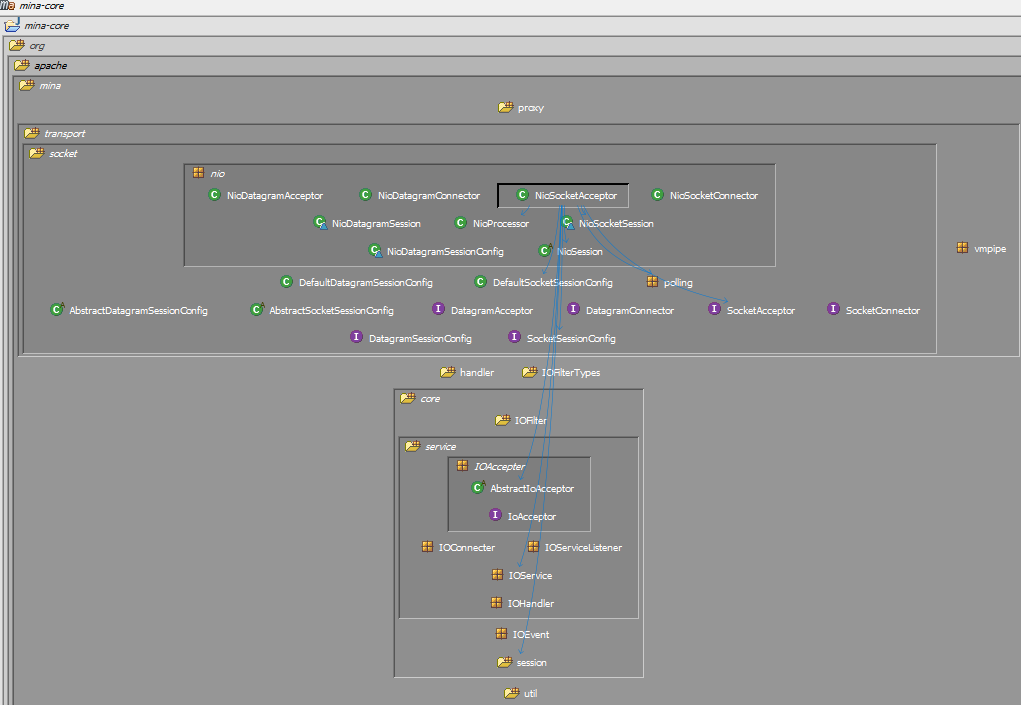
\includegraphics[width=\textwidth]{images/IOacceptor.png}
%     \caption{Architectural implications of step 1 in the server use case.}
%     \label{fig:step1}
% \end{figure}

\underline{\textsc{Step 2}}:\\
The following step is to define a handler, an instance which will react to the communication events between the clients and our server. The responsibility of the handler is to implement the user defined business logic: what actions should be taken when a client connects to the server? or when a message is received?\\\\
The handler needs to be added to the \texttt{connectionsAcceptor}; it will be an user-defined implementation of the \texttt{IOHandlerAdapter} class:

\begin{verbatim}
    // serverHandler extends IOHandlerAdapter
    connectionsAcceptor.setHandler(new serverHandler());
\end{verbatim}

This establishes a connection between packages \texttt{IOAcceptor} and \texttt{IOHandler} via the \texttt{IOHandler} interface.

\underline{\textsc{Step 3}}:\\
Since the server deals with IO communication, MINA offers the possibility of applying filters on the client connections and, therefore, on the inflow/outflow of data. Filters can be chained to obtain the functionality desired by the user.\\\\
Each \texttt{IOAdapter} has a predefined \texttt{DefaultFilterChainBuilder} which creates a corresponding \texttt{FilterChain}; this allows the user to easily add various types of filters to the chain:

\begin{verbatim}
    // adds a new logging filter as the last element of the filter chain
    connectionsAcceptor.getFilterChain().addLast("logging filter", new LoggingFilter());
    /* adds a encoder/decoder protocol filter which transforms message objects 
    *into specific data types
    *TextLineCodecFactory handles text based messages 
    */
    connectionsAcceptor.getFilterChain().addLast("text codec", 
    new ProtocolCodecFilter(new TextLineCodecFactory( Charset.forName( "UTF-8"))));
\end{verbatim}

In this manner, the \texttt{IOService} package is also related to the \texttt{IOFilter} component, which in turn is related to the \texttt{IOFilterTypes} package.

\underline{\textsc{Step 4}}:\\
Whenever a client connection is established with the server, a new session is created by default (more accurately, it becomes active). The acceptor's responsibility is to create and manage this session correspondingly, as well as to notify the handler of the events occurring during the session. This process is part of the inner workings of MINA.\\\\
The user, however, has the option to configure the \textt{IOSession} according to their specifications:

\begin{verbatim}
    // sets the IO buffer size to SIZE
    connectionsAcceptor.getSessionConfig().setReadBufferSize(SIZE);
    // determine acceptable idle time of the connection
    connectionsAcceptor.getSessionConfig().setIdleTime(IdleStatus.BOTH_IDLE, 10);
\end{verbatim}

This directly connects the \texttt{service} and the \texttt{session} packages.







\newpage
\section{Pacito Development}
This section will describe the improvements and changes made in Pacito, and will also list the difficulties we ran into while testing out the tool and its usability aspects.

\subsection{Integrated Pacito}
The main development work done so far is the integration of all components (Pinot, shell scripts, tools) into a single Java executable. This single tool has a link to the native C++ code of Pinot, and will receive the pattern results straight into memory. This way, no output parsing is necessary and everything is contained within a single executable. Some features of the new tool:
\begin{itemize}
    \item Multithreading: Pacito supports multithreading with a predefined number of threads. It will distribute the commits to analyse dynamically using a threadpool in Java, and each thread will have its own independent working directory. This provides fully parallel operation, so it is very well scalable. It is possible to fully analyse a branch of Mina in about 15 minutes on 8 cores.
    \item Use of temporary file system: Pacito will copy the source of the application to a separate working directory, preferably on a {\tt tmpfs} mount, so all file I/O will be done in-memory. This provides significant speed-ups.
    \item User-friendly command-line interface: Pacito as a tool has a nice command-line interface with many options to customise the behaviour
    \item Native integration with Maven: Pacito will integrate straight with Maven and if necessary modify the {\tt pom.xml} files via the API. This ensures that the resulting package download will always succeed and will yield the largest amount of resolved dependencies possible
    \item Maven cache: Each runner thread will use its own Maven cache, to save time downloading resources for each commit.
    \item Native integration with Git: Pacito integrates straight with Git via a third-party library, simplifying the management of the git repository
    \item No Java refactoring necessary: Pacito contains a modified version of Pinot that no longer requires refactoring the source code to analyse
    \item Docker-ready: Pacito can be run in a Docker container, fully hiding all necessary dependencies for the tool to operate. (not yet provided)
    \item Exclude filter: Pacito supports excluding certain directories from the analysis, such as an {\tt examples} directory.
    \item Cross-commit analysis: The set-up of a single integrated program makes it very easy to make intra-commit analyses of the patterns.
\end{itemize}

\subsection{Modified Pinot}
As mentioned before, Pacito contains a modified version of Pinot, with the following improvements:
\begin{itemize}
    \item Support for foreach loops: Pinot can now parse most types of foreach loops, yielding considerably more files to be successfully analysed.
    \item Support for annotations: Pinot can now parse annotations, and will ignore them in further analysis.
    \item More lenient with generics: Pinot does not support generics, and this will often cause a cascade of issues where the generic types cannot be resolved. However, by assuming the source code to analyse is correct, it is possible to make Pinot less strict in its analysis to allow for more files analysed
    \item Fewer memory leaks: Pinot has considerably fewer memory leaks
    \item Redesigned runtime: Pinot has an overhauled public API that better integrates the pattern analysis
\end{itemize}

\subsection{Issues encountered}
During the development of the above features, a number of issues were encountered (very) often, significantly slowing down proper progress and analysis:
\begin{itemize}
    \item Segmentation faults: Pinot is an adapted version of an old open-source Java compiler by IBM: Jikes. This compiler works fine and has memory management done reasonably well, but the changes made by the developer of Pinot make everything into a real tangle where very often freed memory is being accessed again, memory is freed twice, object slicing is happening everywhere, vtables are being corrupted, etc. Every run for every commit is different, and this makes it very hard to debug. On top of that, due to the use of the Java integration, valgrind is very slow since the Java Virtual Machine is causing literally millions of unsolvable errors.
    
    This all makes the program very hard to debug, especially if you want to keep the memory leaks under control. Over time, we managed to reduce the leak from 20MB per commit to about 300kB, which is much more acceptable.
    
    \item Maven not being able to resolve dependencies: Most projects consist of multiple modules, where one depends on the other. In order for Pinot (which requires jars all dependencies) to properly work, we want to supply as many dependency jars as possible. For this, we use the Maven Dependency Plugin, that will copy all these .jar files to a separate directory for us. Unfortunately, this plugin requires the project to be built before the cross-project dependencies can be resolved. This is a consequence of the architecture of Maven.
    
    The original version of Pacito had a tool that would adapt the {\tt pom.xml} files to account for this, but unfortunately, for us it caused a situation where no dependencies could be resolved anymore at all. In the new version, we are using the official Maven API to manipulate the pom files and remove the cross-project dependencies. This allows us to resolve all external dependencies and get their jar files.
    
    \item Pinot not accepting input files. As mentioned before, Pinot is based on the Jikes compiler for which development was discontinued partly through the introduction of JDK5. Consequently, some of the features of JDK5 are implemented, some are not. Luckily, annotations and foreach constructs were already implemented, and we spent some time modifying Pinot to accept these constructs as well.
    
    Unfortunately, the lack of support for generics was causing a number of issues. The lexer and parser of the compiler did already support generics, so the program would not crash; the program would only not parse the files in question. In practice, this causes over half of the classes to not be detected. We tried to circumvent these restrictions in Pinot/Jikes by attempting some workaround, but none of them worked properly.
\end{itemize}
\newpage
\section{Design patterns: identification and analysis}
The section at hand treats the question of introducing, and removing, design patterns in the context of an open source software project, in our case study, the MINA project. MINA has been analysed using the Pacito tool proposed in \cite{pacito}; Pacito has been extended and adapted to better fit our needs as described in section \ref{sec:pacito_dev}. The outcome of applying Pacito on the MINA code base is a dataset which comprises of historical data of design patterns instances which have appeared over the entire commit history of the MINA 2.1.X GitHub branch \cite{mina-github}. This branch corresponds with MINA version 2.1.3 analysed in this report.\\\\
Each entry in the achieved dataset captures one pattern instance identified in the code base and has the following structure:

\begin{verbatim}
    {
        "introCommitName": ,
        "introCommitNumber": ,
        "introCommitMessage": ,
        "outroCommitNumber": ,
        "outroCommitName": ,
        "outroCommitMessage": ,
        "patternName": ,
        "pattern": {},
        "lifespan": ,
    }
\end{verbatim}
The \texttt{introCommit} and \texttt{outroCommit} fields identify the moments in the commit history when the pattern instance has been introduce and, respectively, removed. The \texttt{lifespan} field represents the `life span' of the pattern instance, expressed in number of commits (i.e. from the instance's introduction until its removal). If \texttt{outroCommitNumber} equals \texttt{lastCommitNumber}, then the pattern instance is still current (i.e. still present in the latest version of the code base). The \texttt{pattern} field holds an object which offers more information about the pattern instance. This information is extracted by PINOT \cite{pinot}, which is the building block of the Pacito tool, and varies depending on the pattern type. Generally, information about the pattern instance's code scope is presented (i.e. the  files in the code base that are related to the pattern instance's implementation).\\\\
Our approach to understanding the rationale behind introducing and removing patterns in MINA is to analyse the issue from two perspectives: on one hand, we conduct a quantitative analysis based on the extracted dataset combined with our knowledge of the system and its complexity, on the other hand, we select individual pattern instances from the dataset and cross reference the obtained information from Pacito with other sources (i.e. mailing list, JIRA issues, previous system architectures) in order to gather concrete insight into the decision of introducing or removing patterns. Finally, we combine the results of these two approaches and we conclude. 

\subsection{Data pre-processing}
Prior to analysing the dataset, certain pre-processing steps were required. We observed that Pacito recovers the same pattern multiple times for a specific class due to different properties of the pattern implementation. We decided to merge these occurrences in what we will refer to for the rest of the section as a \textit{pattern instance}. A \textit{pattern instance} is defined by a recovered pattern, a class file (i.e. corresponding to the implementation) and its implementation which can consist of multiple properties. A \textit{pattern instance} is also bounded by an \textit{introCommit} and \textit{outroCommit}. To better exemplify this, if the implementation of a pattern in a certain class changes (e.g. some properties change), a new \textit{pattern instance} will be introduced, while the previous one will be regarded as removed since the code base does not reflect its implementation any longer.\\\\
Another aspect we observed was related to commits \#1850 and \#1851; these commits capture a module refactoring: at commit \#1850 old patterns have been removed and re-introduced at commit \#1851. We cross-matched the recovered patterns at these commits (in accordance to the definition of a \textit{pattern instance}, therefore we also took into consideration the implementation, not only the class file names) and we identified which \textit{pattern instances} 'survived' the module refactoring.\\\\
Before these pre-processing step the dataset contained a total of 2586 recovered patterns, while after the pre-processing, the number dropped to 1882 pattern instances.


\subsection{Recovered patterns dataset analysis}
The recovered patterns dataset includes 1882 data points which represent pattern instances in the MINA code base. Out of the 1882 instances, 1802 have been removed from the project, currently, 80 pattern instances still being included in the stable code base of version 2.1.3. These numbers are not surprising since the entire commit history has been analysed (aprox. 2546 commits out of which 551 commits were relevant to the topic of this analysis), however the number of currently included pattern instances is relatively high, considering the open source nature of the project and that no clear architecture has been initially defined (few mentions about architectural decisions regarding the usage of design patterns in the documentation). Moreover, the significant number of pattern instances removals (almost as large as the number of commits) indicate a fast pace of architectural and implementation changes throughout the development phase. This might lead to a preliminary conclusion that design patterns are introduced out of necessity for solving complex problems and they arise from the experience of the developers, rather than being the blueprint of the software to be developed.
\subsubsection{Overview of recovered patterns \& rate of pattern changes}
Figures \ref{fig:pattern_occ_all}, \ref{fig:pattern_occ_current} and \ref{fig:pattern_occ_removed} present an overview of the occurrence of pattern instances overall, in the current code version of the MINA 2.1.3 project and, respectively, the removed instances. Overall, 15 different patterns have been recovered, currently, 11 out of the 15 are present. Following the GoF (Gang of Four) \cite{gof} design pattern classification, most patterns used are either structural (e.g. Decorator, Facade, Adapter, Bridge, Flyweight) or behavioural (e.g. Strategy, Mediator, Observer, Chain of Responsibility, Template, Visitor). The most used patterns are, by far, the Strategy and Mediator patterns. 
\begin{figure}
    \centering
    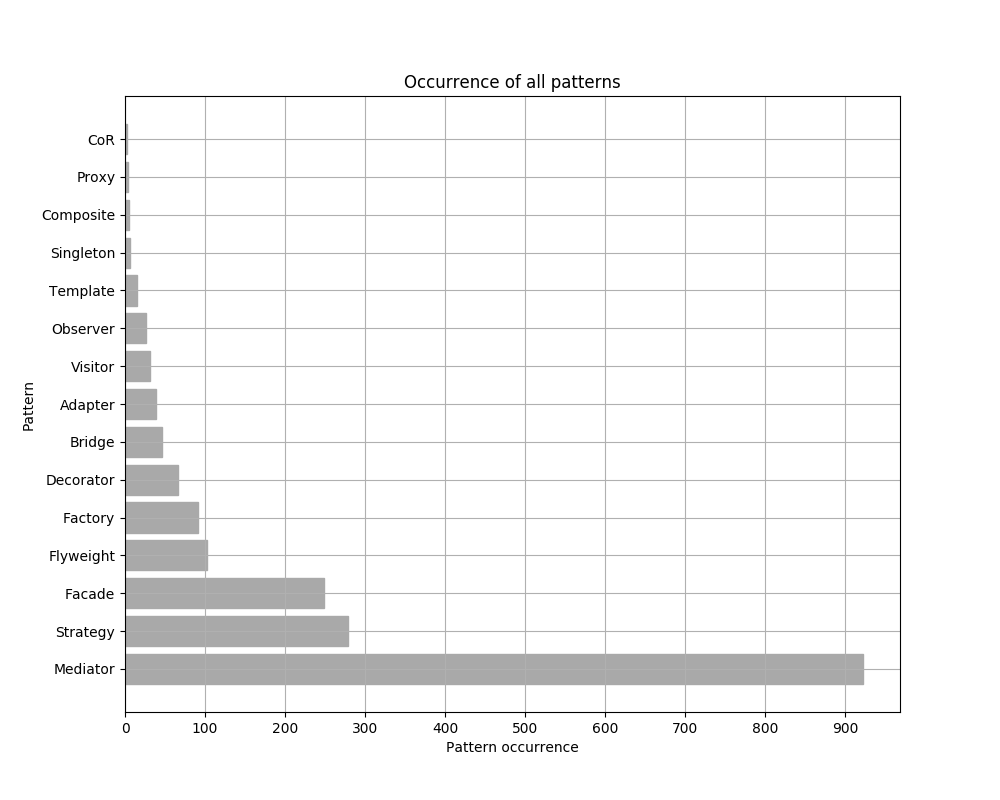
\includegraphics[width = \textwidth]{images/graphs/pattern_occurrence_all.png}
    \caption{Overview of all pattern instances retrieved from the entire commit history of MINA 2.1.3. 15 different patterns have been introduced, with the \texttt{Mediator} and \texttt{Strategy} pattern having the most occurrences.}
    \label{fig:pattern_occ_all}
\end{figure}
\begin{figure}[H]
    \centering
    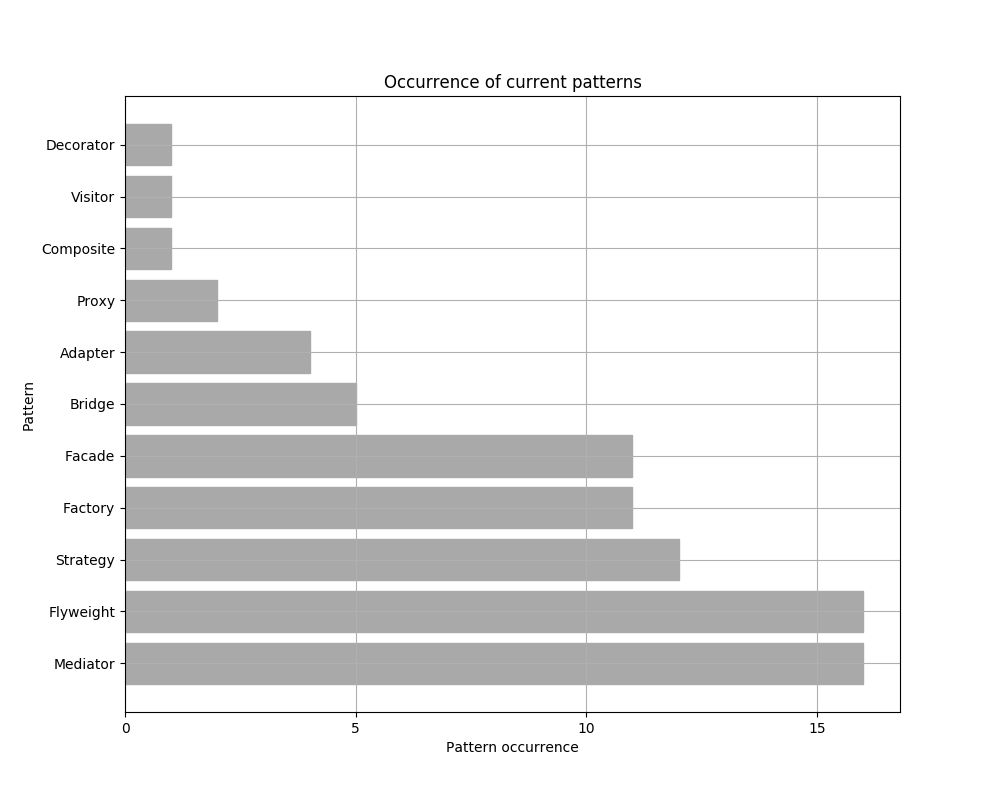
\includegraphics[width = \textwidth]{images/graphs/pattern_occurrence_current.png}
    \caption{Overview of current pattern instances in the latest code base version of MINA 2.1.3. 11 patterns are still kept from the overall 15 presented in figure \ref{fig:pattern_occ_all}, with the \texttt{Mediator} and \texttt{Fylweight} patterns having the most occurrences.}
\label{fig:pattern_occ_current}
\end{figure}

\begin{figure}
    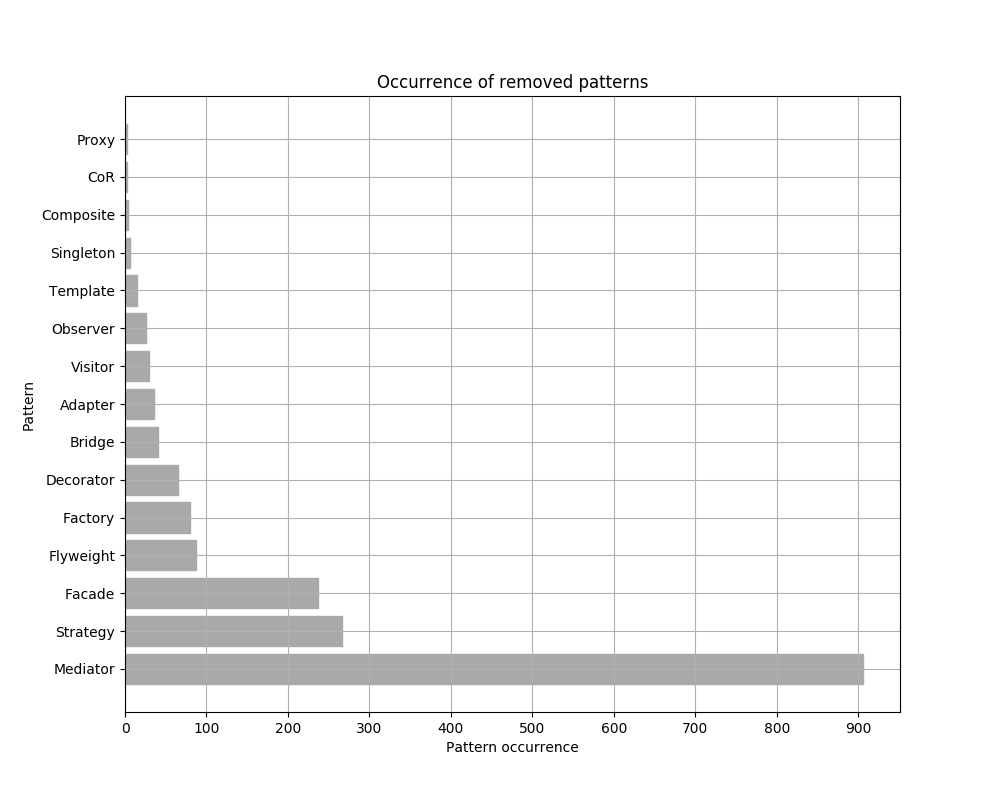
\includegraphics[width = \textwidth]{images/graphs/pattern_occurrence_removed.png}
    \caption{Overview of removed pattern instances; most of the pattern instances with a high occurrence, as presented in figure \ref{fig:pattern_occ_all}, have been removed (i.e. aprox. 900 instances of the \texttt{Mediator} pattern have been removed}.
 
  \label{fig:pattern_occ_removed}  
    
\end{figure}

The Strategy pattern allows the choice of an algorithm at run time from a family of previously defined algorithms. In the context of MINA, this pattern could be suitable in multiple instances, for example for the transport, filtering and handler components. The Mediator pattern allows loose coupling between classes by enabling interaction that do not require the participating classes to have any knowledge of each other. This pattern achieves high modifiability through encapsulation and could have been applied anywhere in the scope of the MINA project. The striking large number of occurrences of these two patterns (especially for the Mediator pattern which is recovered more than 900 times over the entire project) is tackled by an equally large number of removals (i.e. aprox. 900 removals for the Mediator pattern, see figure \ref{fig:pattern_occ_removed}) which shows the superfluous nature of introducing patterns in cases that do not fit the pattern context. This also points to a tendency towards redundancy in the development of MINA. \\\\
The variation between introducing and removing patterns is also captured by figure \ref{fig:per_removed_patterns}. Out of the total number of pattern instances recovered with Pacito, 95.7\% of them have been removed. This re-enforces our previous statement that the patterns in discussion have been introduced after establishing the initial architecture, following rather a trial and error strategy, rather than a pattern driven model for architecture modelling (for example, the proposed PDAP methodology proposed in \cite{pdap}). Even though design patterns offer proven solutions to complex, reoccurring problems, they inherently require more attention to implementation and imply certain trade-offs or implications. These implications of introducing patterns \textit{a posteriori} might have led to the high variation between additions and removals, for example issues such as increased code complexity, cross cutting concerns, increased development and maintenance time might have been potential reasons for pattern removals. 
\begin{figure}
    \centering
    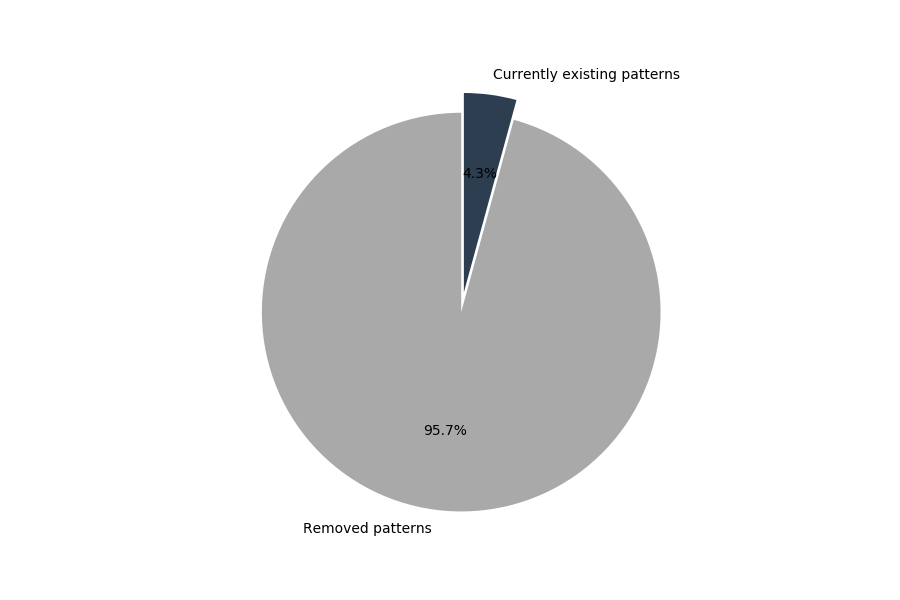
\includegraphics[width =  \textwidth]{images/graphs/current_removed_per.png}
    \caption{Percentage of removed pattern instances out of all recovered patterns.}
    \label{fig:per_removed_patterns}
\end{figure}

The mean lifespan, expressed in number of commits, of the identified patterns is presented in figure \ref{fig:mean_life}. From the figure, it is apparent that the mean lifespan of the Proxy pattern instances is an outlier. For this graph, we must consider that Pacito  accounts for 'gaps' between removal and a new addition of the same pattern instance, which results into significantly large values. The existence of 'gaps' offers insights into the inconsistencies in development: a decision to add, remove and then add again a pattern instance for the same scope of the project is proof of the fragmented thought process of the development community. However, this is not out of the ordinary for an open software project which implies a volatile development team structure and lack of centralized decision making. The median 'life expectency' of a pattern instance is of aprox. 50 commits, which is aprox. 9\% out of the total number of commits made. This can be translated into a high velocity of structural changes.

\begin{figure}[H]
    \centering
    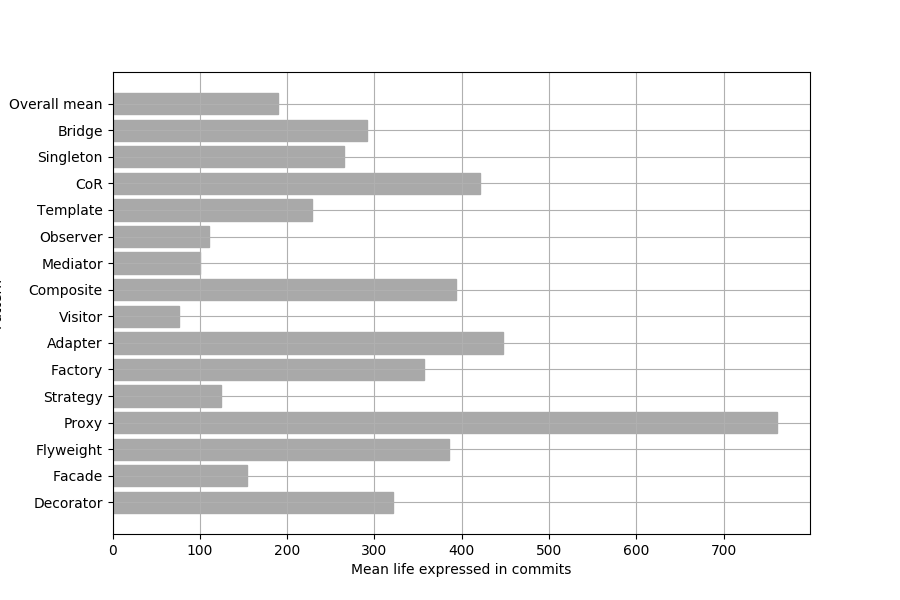
\includegraphics[width =  \textwidth]{images/graphs/mean_life.png}
    \caption{Median lifespan expressed in commits for the removed patterns.}
    \label{fig:mean_life}
\end{figure}

\subsubsection{Rate of pattern introductions and removals at commit level}
The commit history analysed can be classified into 3 categories: commits which introduce new pattern instances (i.e. intro commits), commits which remove existing pattern instances (i.e. outro commits) and the combination of the two (i.e. intro/outro commits). The distribution of the 3 commit types over the entire extracted dataset is presented in figure \ref{fig:pattern_commit_percentage}. The percentage of intro and outro commits are aprox. equal (i.e. 44.3\% and 40.5\%, respectively); this can be regarded as an indicator that most of the pattern instances introduced have been invariably removed after a period of time (see figure \ref{fig:mean_life}). Keeping in mind the large number of pattern instances recovered (i.e. 1882 pattern instances), we reach our second preliminary conclusion that, in the context of MINA, a quantitative rather than a qualitative approach has been taken w.r.t. the patterns used (one might argue that this volatility could have been influenced by changes in requirements, however, we will show in section \ref{sec:scope_analysis} that the scopes of most of the patterns overlap with the \texttt{core} component of MINA which has been stable in terms of features/functional requirements since its initial version).  
\begin{figure}[H]
    \centering
    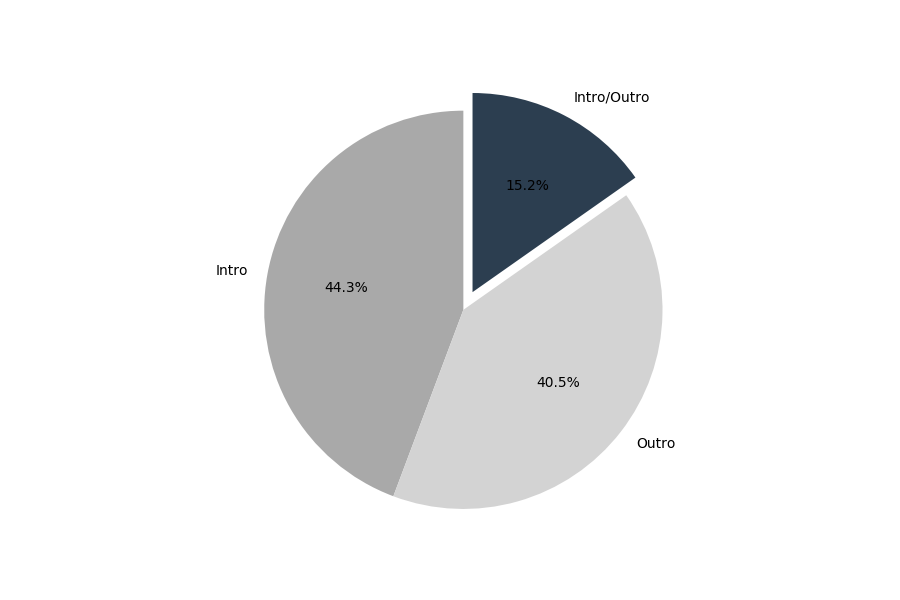
\includegraphics[width =\textwidth]{images/graphs/intro_outro_per.png}
    \caption{Distribution of pattern instances introductions and removals over the analysed commits.}
    \label{fig:pattern_commit_percentage}
\end{figure}
The intro/outro commits imply additional complexity: a pattern instance removal is followed by the introduction of a more suitable pattern, for example. Figure \ref{fig:add_rem_commit} shows an account of pattern introductions and removals per commit. The visualisation capture the workflow of the development team which corresponds to small and more frequent commits. As predicted from the previous figure, the (0, y) axis (corresponding to outro commits) is similar to the (x, 0) axis (corresponding to intro commits), the most evident difference is that intro commits are spread in the [0, 30] interval (more focused in the [0, 15] interval) and can span up until over 30 additions per commit (commits exceeding this bound are considered outliers). The outro commits also span the [0, 30] interval, but increase consistently. Pattern removals are therefore more consistent and iterative, while additions are generally kept towards the lower bound, but can appear sporadically and have a greater impact by introducing a large number of pattern instances at once. The intro/outro commits are bounded by the 15 additions/removals limit. Given this bound, their impact is comparatively less significant, therefore they might be intended for improvements or switching patterns for more suitable alternatives, while still preserving the global pattern occurrences. 
\begin{figure}[H]
    \centering
    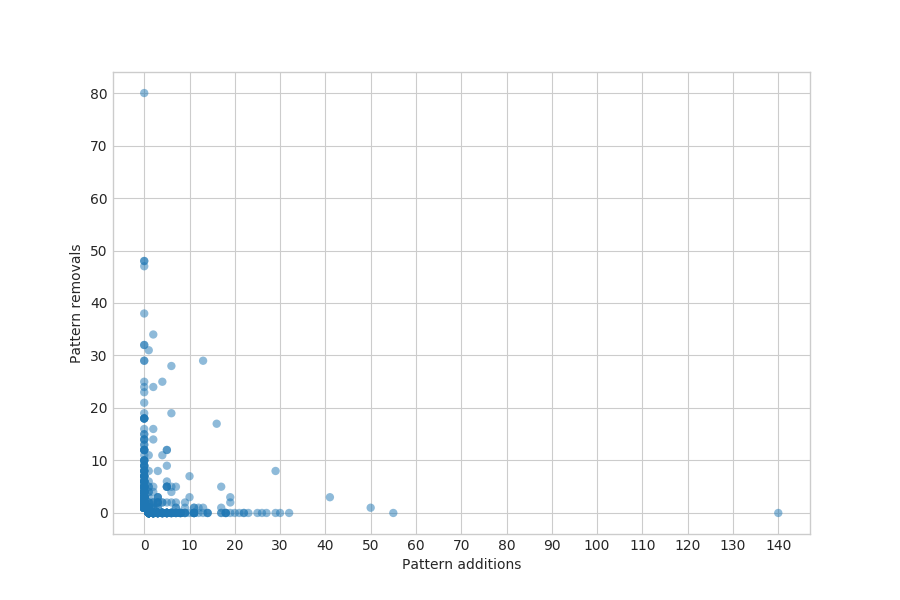
\includegraphics[width =\textwidth]{images/graphs/additions_removals_commit.png}
    \caption{Pattern instances additions and removals per commit.}
    \label{fig:add_rem_commit}
\end{figure}

Figure \ref{fig:commit_timeline} presents a timeline of the evolution of the total number of patterns in the code base in accordance with the analysed commits. The pattern data shows as descending trend; the peak was reached around commit \#300 (roughly capturing the start of the development phase of MINA version 1.0.0), reaching a plateau-like state around commits \#1500 - \#2300; most recently, following a decrease below 100 patterns. This decrease shows a tendency towards stabilization, which follows from the fact that the project is reaching towards its maturity (already version 2.1.3). The phase when much of the volatility and changes in terms of patterns seem to have occurred is the period between commit \#600 and \#1200 - \#1500 (which roughly correspond to the development of versions 2.0.X).  

\begin{figure}[H]
    \centering
    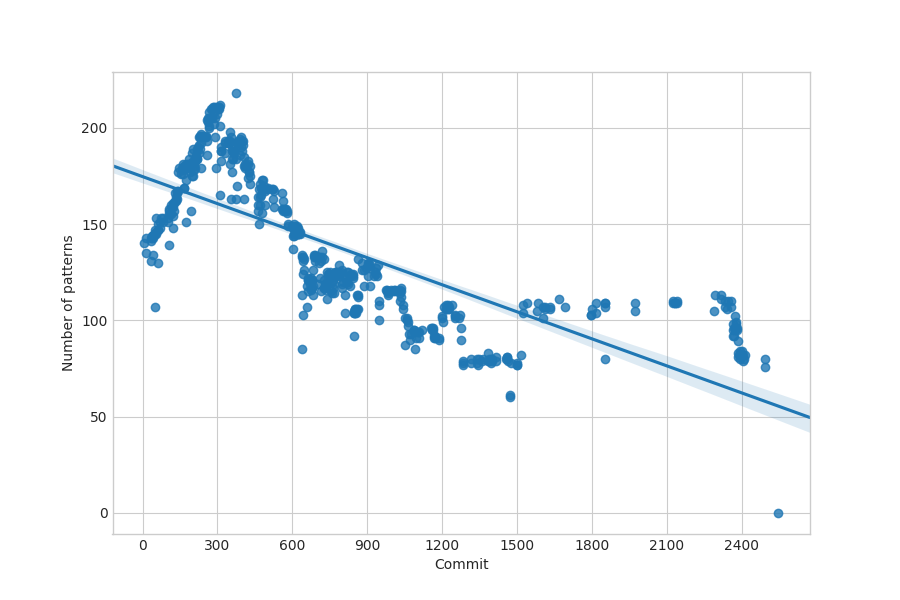
\includegraphics[width =\textwidth]{images/graphs/commit_timeline.png}
    \caption{Timeline of analysed commits as expressed by the total number of pattern occurrences at the time of the commit. The timeline is fitted with a linear regression.}
    \label{fig:commit_timeline}
\end{figure}

\subsubsection{Distribution of patterns over the MINA components scope}
\label{sec:scope_analysis}
Design patterns are usually introduced for the main purpose of facilitating the implementation of a proven to a complex, reoccurring problem. This leads to the investigation of the scope of the introduced patterns: by understanding \textit{where} they have been introduced, one might be able to infer the \textit{why}. Figure \ref{fig:scope_percentages} shows the distribution of all the patterns recovered in accordance to their implementation scope within the MINA code base (namings might different since the entire commit history has been considered). Figure \ref{fig:others_scope_percentages} complements figure \ref{fig:scope_percentages}. The most prominent component is the \texttt{core}; as described in section \ref{sec:analysis_components}, it is the backbone of MINA and offers the basic functionalities required to implement a MINA based application. Having the most patterns concentrated over this component is not surprising, since it is also the most extensive component.

\begin{figure}[H]
    \centering
    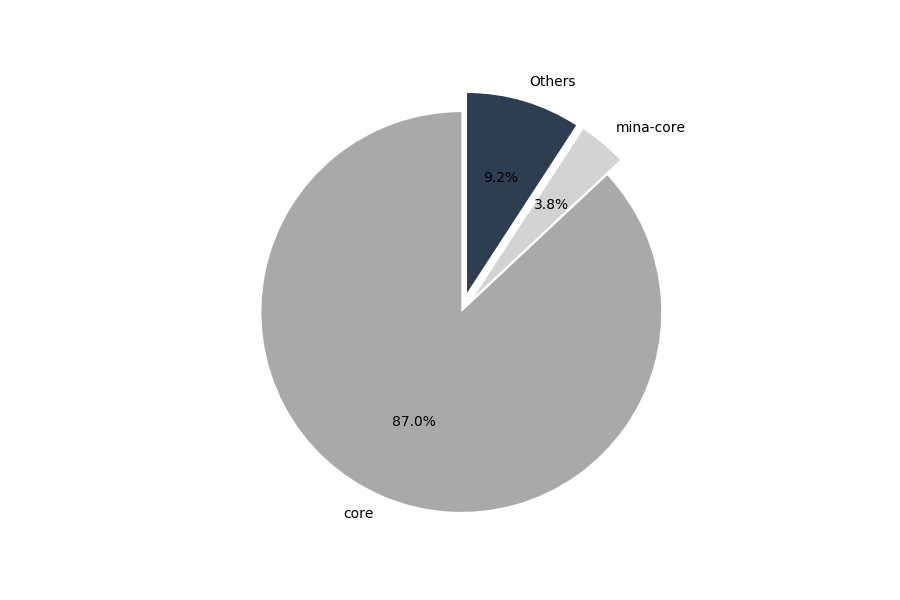
\includegraphics[width =\textwidth]{images/graphs/all_scopes_per.png}
    \caption{Code base component scopes of the recovered patterns from the entire commit history.}
    \label{fig:scope_percentages}
\end{figure}
Other components that entail a significant complexity are the ones implementing the \texttt{http} support (patterns such as Proxy, Strategy could be considered here)  and the \texttt{integration} modules (patterns such as Facade would be suitable in this case). The \texttt{mina-statemachine} component also entails a high level of complexity since it aims at implementing an improved version of the State pattern. 

%% to be changed/moved to appendix
\begin{figure}[H]
    \centering
    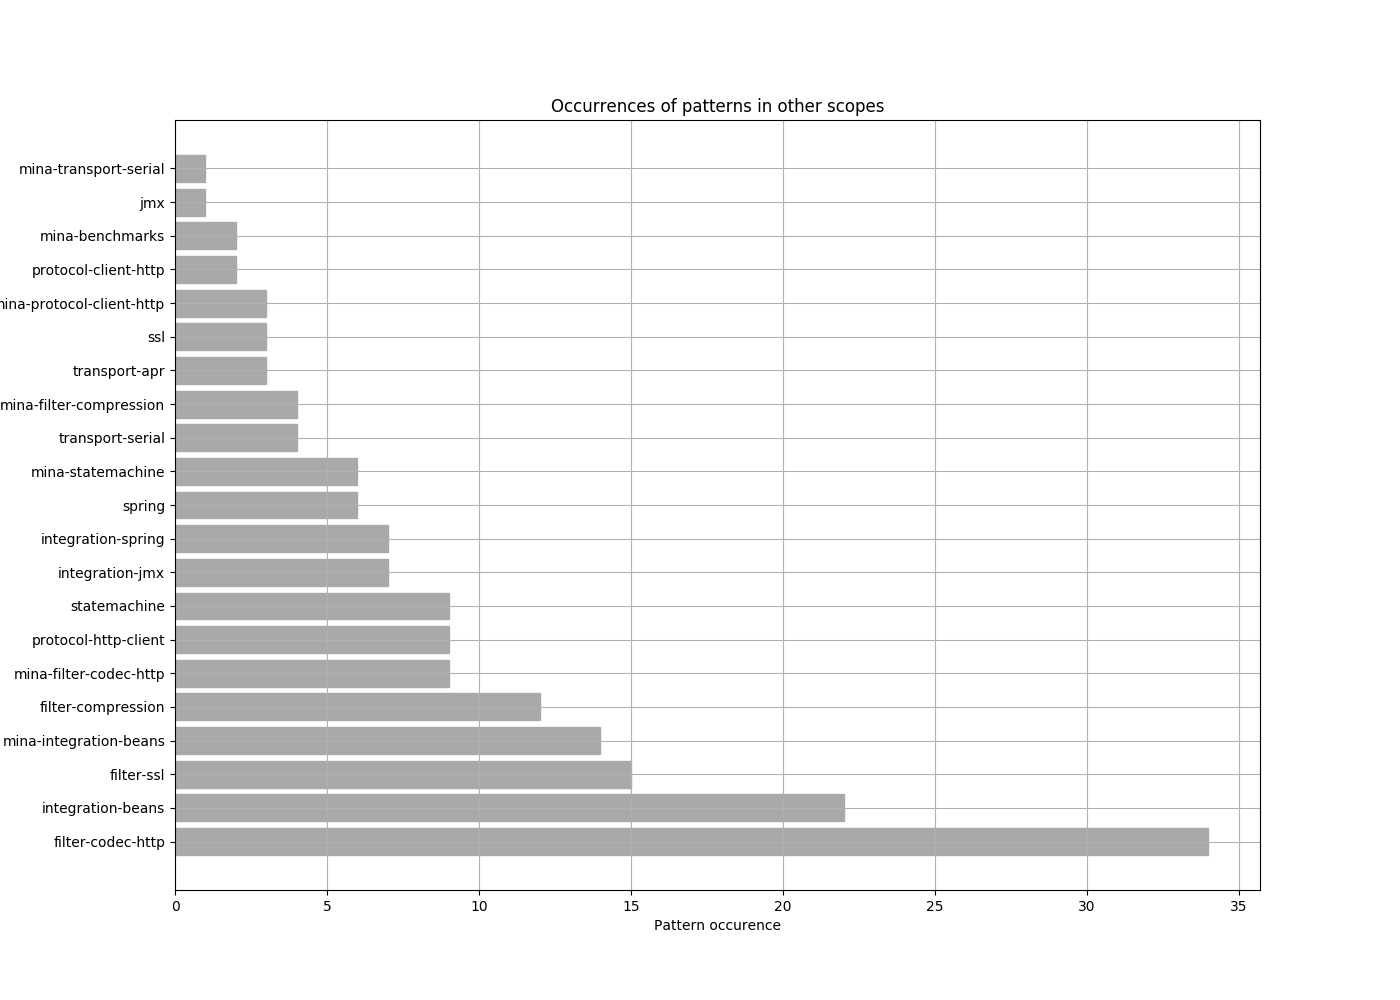
\includegraphics[width = \textwidth]{images/graphs/other_scopes.png}
    \caption{Pattern distribution over "others" scopes, excluding the core component.}
    \label{fig:others_scope_percentages}
\end{figure}

The pattern distribution in the current code base version of MINA is reflected in figure \ref{fig:current_scopes_percentages}. The information depicted in this figure follows the overall pattern distribution presented in the figures above (figures \ref{fig:scope_percentages} and \ref{fig:others_scope_percentages}). Some changes are apparent: for instance, there is no recovered pattern spanning the \texttt{http} related components any more. This might be an indication of the fact that the actual implementation has strayed from the expected pattern implementation, even though the concept is still followed. This might come as a consequence to the fact that design patterns require a certain level of knowledge and understanding in order to achieve a successful implementation. Also, some integration components (i.e. \texttt{jmx}, \texttt{spring}) are no longer supported by patterns (their complexity might have been overestimated).
\begin{figure}[H]
    \centering
    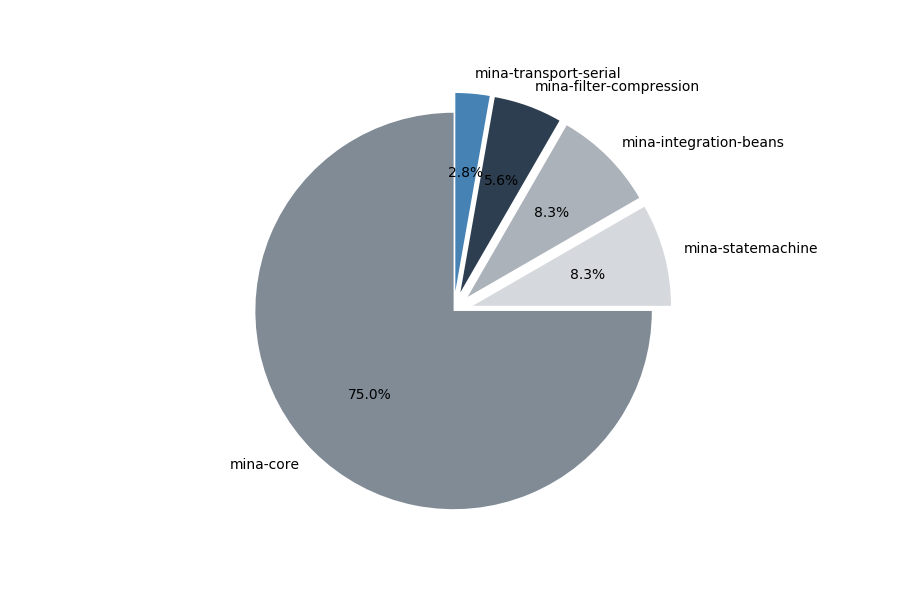
\includegraphics[width =\textwidth]{images/graphs/current_scopes_per.png}
    \caption{Distribution of current pattern instances over all the components of the MINA project. \texttt{mina-core} includes the \texttt{core} component.}
    \label{fig:current_scopes_percentages}
\end{figure}

Figure \ref{fig:mina_core_scope} narrows the scope to more specific areas of the code base where current patterns exist. From this diagram, the intricacy of the component implementation becomes clear: the most occurrences appear over components that support the implementation of the \texttt{filter} components; following the component descriptions in section \ref{sec:analysis_components}, through the \texttt{filtering} components,  additional functionality of processing networking communication is provided. Since various filters of different complexities are provided out-of-the-box, it follows logically that the filtering components would require more attention to tackle the various complexities entailed. Components that support the networking \texttt{transport}, as well as the \texttt{service} and \texttt{session} components, are also spanned by multiple pattern occurrences; these are complex components that bind together all necessary elements for establishing the baseline connection between client and server, which resides at the backbone of any networking application. The \texttt{byteaccess} component contains the most pattern occurrences, respectively 8 pattern instances; this follows from the fact that basic data buffers are implemented from scratch in MINA.

\begin{landscape}
\begin{figure}
    \centering
    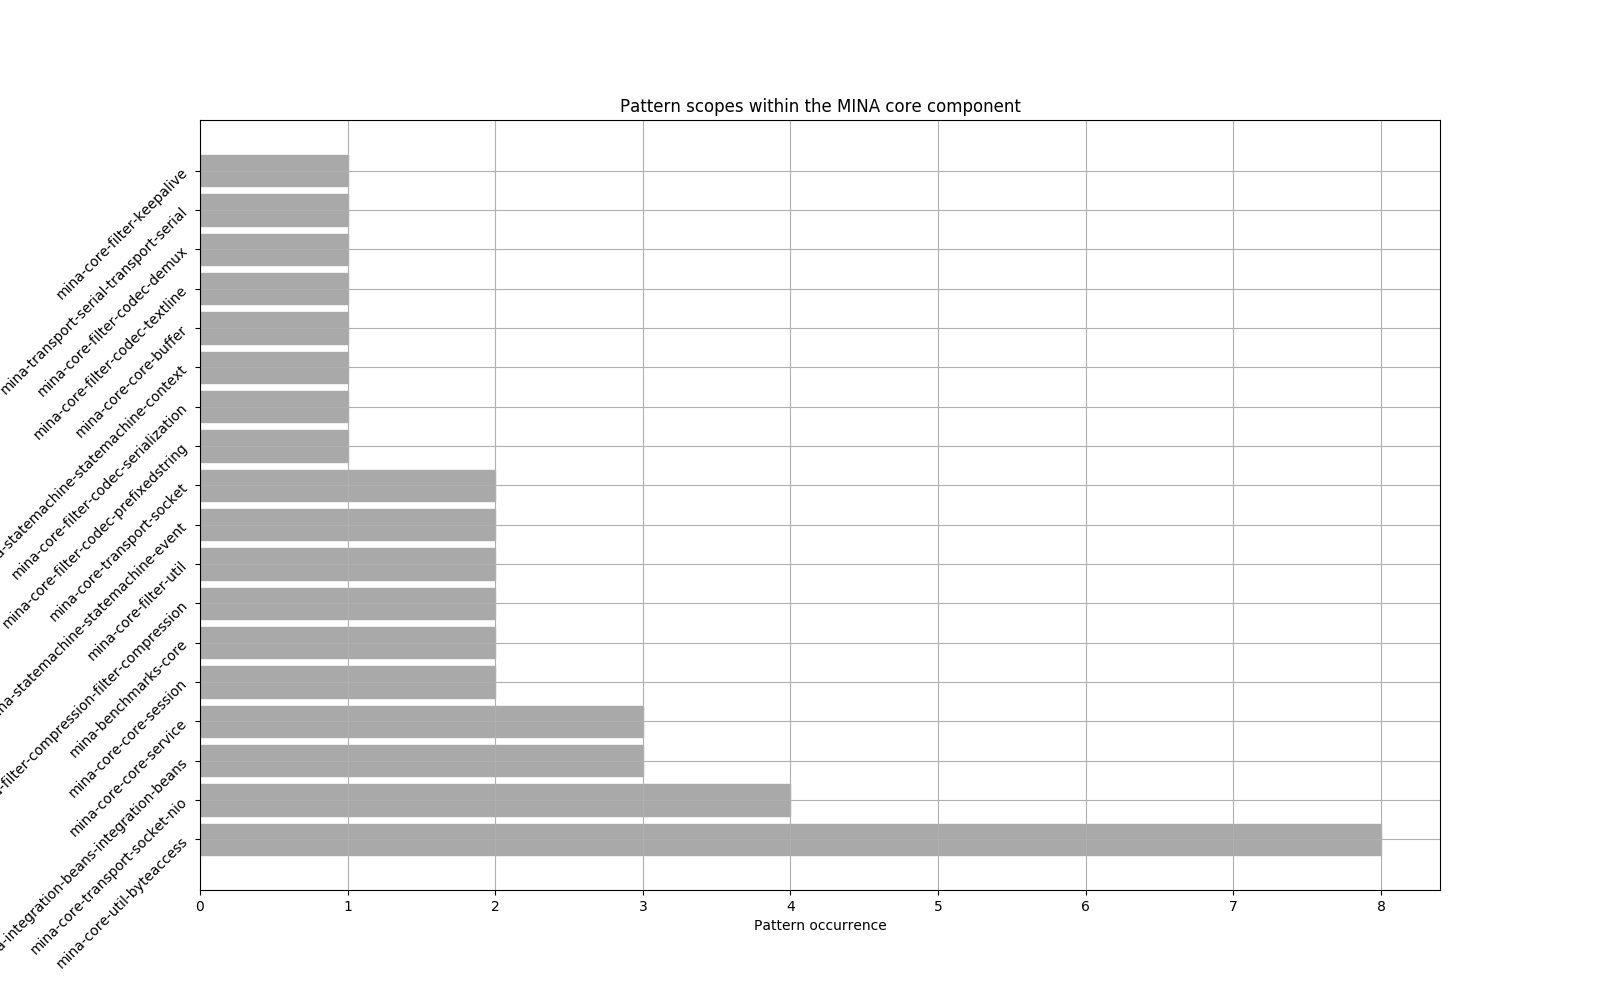
\includegraphics[scale = 0.6]{images/graphs/core_scopes.png}
    \caption{Overview of the current patterns w.r.t. the current components of MINA.}
    \label{fig:mina_core_scope}
\end{figure}
\end{landscape}

\subsection{Individual patterns analysis}
Following the quantitative analysis, we investigate a sample of recovered pattern instances individually. The sample includes both patterns that have been removed, as well as patterns that are currently implemented in the code base. The key aspects relevant to this investigation are the implementation of the patterns \footnote{We judge the Java implementation starting from the pattern definition for which we use online sources that are available to any developer; we assume that no academic understanding of design patterns is required}, as well as the motivation behind their introduction, and possible removal. The impact on the overall architecture (as presented in section \ref{sec:analysis_components}) is also considered.

\subsubsection{Current patterns: Facade \& Adapter patterns}
\label{sec:current_facade_adapter}
The implementation of the out-of-the-box prefixed codec filter uses both the Facade and Adapter patterns, as recovered by Pacito. We present and analyse these patterns as a whole as follows:\\\\
\textsc{Pattern definition}: 
\begin{itemize}
    \item \textsc{Facade} is a structural pattern which hides the complexities of a system by providing a simplified interface to said system. Implementation wise, Facade implies a single class or point-of-entry to the system which communicates with the user (or client) and provides simplified methods by delegating to underlying classes that are not directly visible to the user \cite{facade}\cite{facade1}.
    \item \textsc{Adapter} combines the functionalities of independent interfaces; it is also considered a structural pattern since it provides a means of communication between separate structural entities. It entails an adapter and adaptees: the adapter wraps the functionality of the adaptees in order to facilitate the service usage of the adaptees by an independent, incompatible client entity \cite{adapter}\cite{adapter1}.
\end{itemize}
\textsc{Pattern implementation information from Pacito}: 

\begin{itemize}
    \item Pacito has identified 2 Facade pattern instances which are complementary to one another; we present them together:
        \begin{itemize}
            \item \textsc{Access point}: \texttt{PrefixedStringCodecFactory}
            \item \textsc{Facade}: \texttt{PrefixedStringEncoder}, \texttt{PrefixedStringDecoder}
            \item \textsc{Hidden complexity}: \texttt{IOBuffer}, \texttt{ProtocolEncoderOutput}, \texttt{ProtocolDecoderOutput}
            \item \textsc{Scope}: \texttt{mina-core/filter/codec/prefixedstring/}
        \end{itemize}
    \item The Adapter pattern has been recovered twice for two adaptees (which coincide with the facades mentioned above) and one adapter:
        \begin{itemize}
            \item \textsc{Adapter class}: \texttt{PrefixedStringCodecFactory}
            \item \textsc{Adaptees}: \texttt{PrefixedStringEncoder}, \texttt{PrefixedStringDecoder}
            \item \textsc{Adapting}: \texttt{ProtocolCodecFactory}
        \end{itemize}
\end{itemize}
\textsc{Implementation \& class diagram}: The implementation is capture by figure \ref{fig:cd_facade}; the hidden complexity, as captured by Pacito, consists of the results of the prefixed encoding and decoding, as well as the \texttt{IOBuffer} which 'stores' this data. These complexities are wrapped by the corresponding classes (i.e. \texttt{PrefixedStringEncoder} and \texttt{PrefixedStringDecoder}) which encapsulates them in the \texttt{encode} and, respectively, \texttt{doDecode} methods. These 2 classes cannot be directly accessed; they are created by the \texttt{PrefixedStringCodecFactory} which acts as the entry point: a user would interact with this class in order to use the functionality provided by the prefix codec. However, the \texttt{PrefixedStringCodecFactory} does not provide the additional layer of abstraction of delegating responsibilities to its underlying components: this implies that the user needs to be aware of the \texttt{encode} method of the \texttt{encoder} field of the \texttt{PrefixedStringCodecFactory} class in order to access the prefix encoding functionality. This also holds for the decoding step. \\\\
At the same time, the \texttt{PrefixedStringCodecFactory} is identified to be the adapter class which entails that it bridges incompatible interfaces; this recovery is an \textbf{incorrect detection} of the Adapter pattern. We motivate this statement as follows: the adaptees are identified as the \texttt{PrefixedStringEncoder} and \texttt{PrefixedStringDecoder} (they represent implementations of the \texttt{ProtocolEncoder} and \texttt{ProtocolDecoder} interfaces), therefore the \texttt{PrefixedStringCodecFactory} wraps these two classes in order to make them compatible to the adapting interface, \texttt{ProtocolCodecFactory}. However, the \texttt{PrefixedStringCodecFactory} implements \texttt{ProtocolCodecFactory} which, at the same time, has dependencies to the \texttt{ProtocolEncoder} and \texttt{ProtocolDecoder} interfaces. We, however, consider that the \texttt{PrefixedStringCodecFactory} is an instance of the Factory design pattern (as suggested by the name of the class) \cite{factory}: the \texttt{PrefixedStringCodecFactory} creates instances of the \texttt{PrefixedStringEncoder} and \texttt{PrefixedStringDecoder} interfaces.    \\\\
\textsc{Issue tracking \& motivation}: The motivation for the patterns addition is the implementation of a fixed-length prefix encoding/decoding mechanism, where no additional information of delimiters between encoded values is necessary. Moreover, the prefixed codec should be accessible as an out-of-the-box filter for the users developing their MINA based applications. We have identified 18 mentions in the official developer mailing list \cite{mina-mail} regarding the prefix codec which generally discuss the implementation of the codec, however, there is no direct mention of the Facade pattern in relation to this implementation (the keyword 'facade' has been found 43 times, however, it broadly refers to the design pattern and it is found in relation with the logging SLF4J \cite{slf4j} functionality of MINA). As for the adapter pattern (identified by keyword 'adapter'), there is no mention of it w.r.t. the prefixed codec, however, we have identified an extensive discussion within the developers' mailing thread regarding the confusing naming of files (file names contain the 'adapter' keyword) in the absence of the adapter pattern named in the file name. Excerpts from the mailing lists show that the understanding (and/or discussion about the implementation) of the real pattern is limited: \\\\
\textit{"The *Adapter classes are convenience wrappers meant to be extended by the user if he only wants to use a "subset" of the interfaces they implement."}\\\\
\textit{"Again, these classes are \_not\_ adapters, wrt the definition of the 
adapter pattern."}\\\\
\textsc{Impact on architecture}: The impact of the Facade and Adapter patterns on the structure of the overall architecture is not too significant since the scope of the patterns is rather self-contained and does not go beyond the \texttt{mina-core-filter} component. The same approach of using this combination of patterns is also identified for other types of filters within the same component, for example \texttt{ObjectSerializationCodecFactory} and \texttt{TextLineCodecFactory}, which also represent out-of-the-box implementations for processing communicated data.\\\\
\textsc{Preliminary conclusions}: The recovered instance analysed above can be considered a loose implementation of the Facade pattern, where the main goal seems to have been abstraction of complexity, with less focus on how to delegate this complexity such that the user is only coupled with a very simple system entry point. The lack of mentions and discussion about this topic points out to the possibility that the Facade pattern instance, in this specific case, might not have been intentional, but logically followed from respecting good object oriented Java practices, also considering that the Facade pattern does not entail a lot of complexity in itself. As for the Adapter pattern, the two interfaces that are being bridged (as recovered by Pacito) are connected through a dependency, therefore we cannot state that they are completely incompatible. The main motivation behind the adapter, in this particular case, was to expose and provide compatibility for the out-of-the-box codec implementation to the users and their MINA based applications, however this does not yield a correct implementation of this pattern, especially considering the pattern components identified by Pacito. \textbf{In this case, we can state that Pacito has incorrectly detected the Adapter pattern}. Instead, the adapter class can be seen as a good example of a Factory pattern instance. 

\begin{figure}
    \centering
    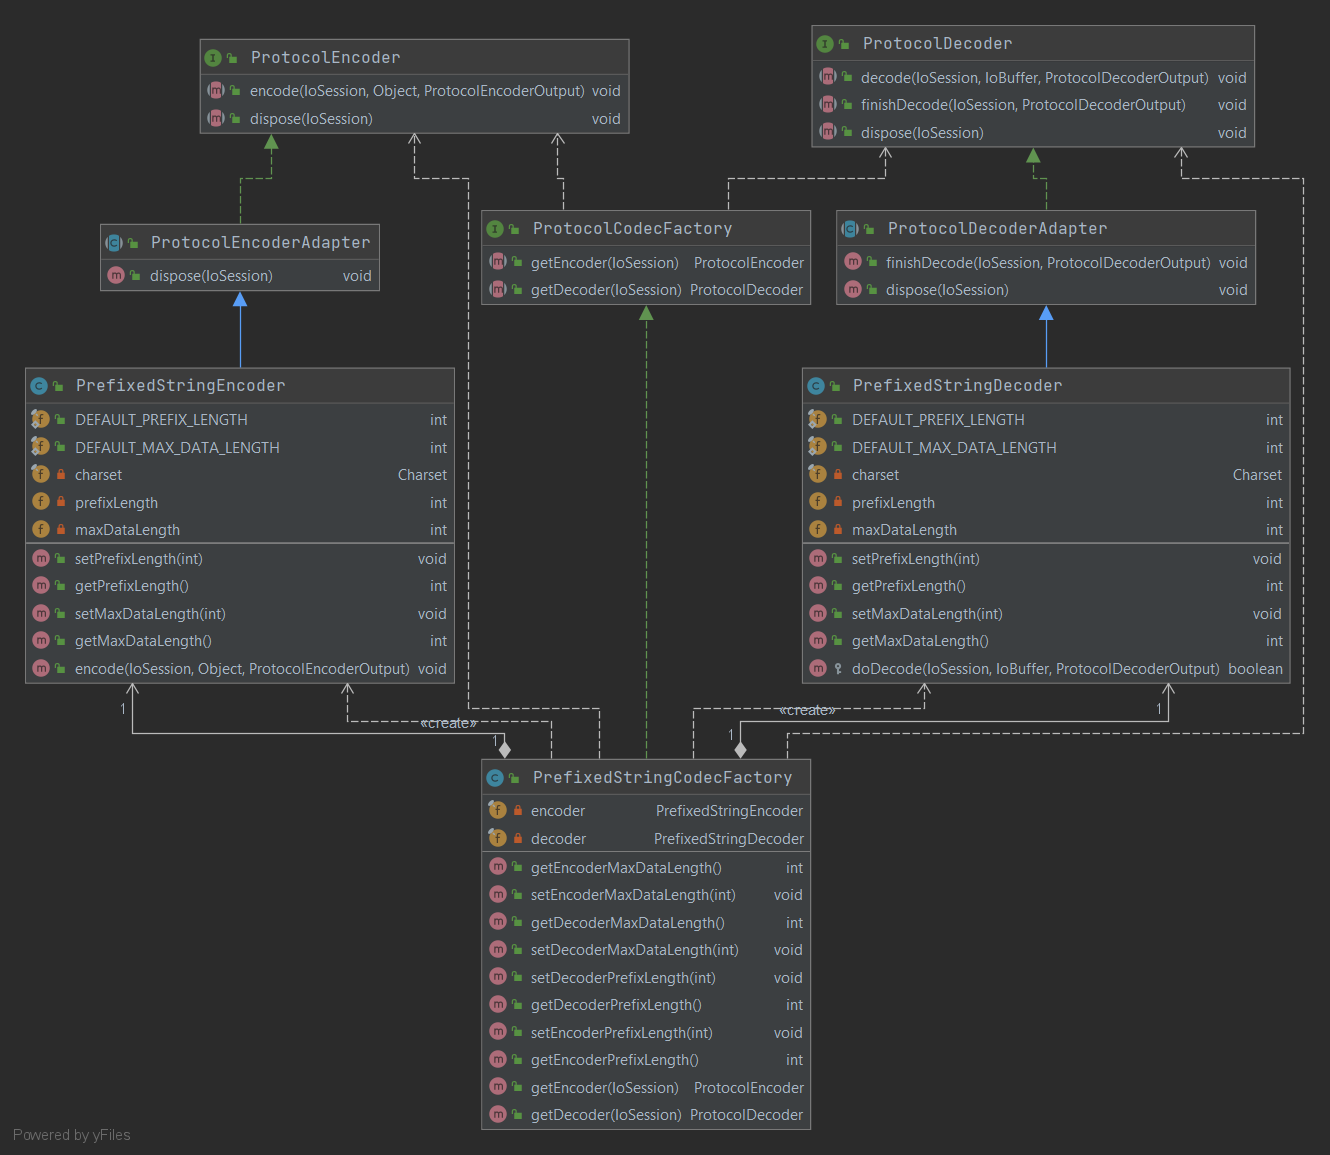
\includegraphics[width = \textwidth]{images/class_diagrams/adapter_facade_pattern.png}
    \caption{Class diagram for the implementation of the Facade and Adapter patterns within the scope of the prefix codec filter.}
    \label{fig:cd_facade}
\end{figure}

\subsubsection{Current patterns: Factory pattern}
The above section presented an instance where the Factory pattern was incorrectly recovered as the Adapter pattern; we, thus, present 2 distinct instances of the Factory pattern where the pattern is correctly represented in the code base.\\\\
\textsc{Pattern definition}: The \textsc{Factory} pattern falls into the category of creational patterns and is one of the most used pattern in OO languages. This pattern provides an interface for creating objects in a superclass, while still allowing for the subclasses to alter the type of objects to be created. The creation logic is not exposed, the newly created objects can be referred to via the said interface \cite{factory}\cite{factory1}.\\\\
\textsc{Pattern implementation information from Pacito}
\begin{itemize}
    \item \textsc{Factory instance 1}
        \begin{itemize}
            \item \textsc{Factory Method Class}: \texttt{StateContextFactory}
            \item \textsc{Factory Method Result Base}: \texttt{StateContext}
            \item \textsc{Factory Method Implementation}: \texttt{DefaultStateContextFactory}
            \item \textsc{Factory Method Results}: \texttt{DefaultStateContext}
            \item \textsc{Factory Method}: \texttt{create}
        \end{itemize}
    \item \textsc{Factory instance 2}
          \begin{itemize}
            \item \textsc{Factory Method Class}: \texttt{ByteArrayFactory}
            \item \textsc{Factory Method Result Base}: \texttt{ByteArray}
            \item \textsc{Factory Method Implementation}: \texttt{SimpleByteArrayFactory}
            \item \textsc{Factory Method Results}: \texttt{BufferByteArray}
            \item \textsc{Factory Method}: \texttt{create}
        \end{itemize}
\end{itemize}
\textsc{Implementations \& class diagrams}: The implementations of the Factory instances are presented in figures \ref{fig:factory1}, \ref{fig:factory2}. The specific factories (i.e. \texttt{DefaultStateContextFactory} and \texttt{SimpleByteArrayFactory}) implement the main Factory interface (i.e. \texttt{StateContextFactory} and \texttt{ByteArrayFactory}) and encapsulate the creation of specific objects, in this case \texttt{DefaultStateContext} and \texttt{BufferByteArray}, which are implementations of a superclass interface, \texttt{StateContext} and \texttt{ByteArray}, respectively. \\\\
\textsc{Issue tracking \& motivation}: The objects that are being created in both cases are meant to be used unaltered in order to ensure that the desired functionality of MINA. In the \texttt{byteaccess} context, the client should not be involved with the creation of the \texttt{BufferByteArray} objects since it cannot accept alterations: the \texttt{BufferByteArray} is part of the MINA specific low level API which uses custom byte buffers. Same situation goes for the \texttt{mina-statemachine} context: the \texttt{DefaultStateContext} object represents the default implementation of a \texttt{StateContext} which implies that it needs to inherit all the required aspects (i.e. stores the current state and all client specific information since all clients use the same \texttt{StateMachine} which is a Singleton) for the successful implementation of the state machine (see section \ref{sec:analysis_components}). Unlike the previous pattern discussed up until this point, the Factory pattern is well discussed between the developers of MINA. It also appears in relation with the 2 instances we discuss here. For the Factory pattern, the developers seem to be aware of the correct implementation of this pattern, as well as of its usage compatibility in various areas of the code base. This remark is also supported by the coherent naming of the factory files. The Factory pattern is most of the times mentioned in relation with codecs, however Pacito does not recover any current Factory instance within the \texttt{mina-filter} scope. An example of a mis-identification of the Factory pattern is mentioned in section \ref{sec:current_facade_adapter}.\\\\
\textsc{Impact on architecture}: The Factory instances presented do not have a significant impact on the overall architecture, however, the approach of using the Factory method for creational purposes spreads over multiple components in the current version of the code base (i.e. \texttt{mina-statemachine}, \texttt{mina-integration}, \texttt{mina-core-transport}, \texttt{mina-core-util}, \texttt{mina-core-IOFilterTypes}). From investigating the code and the developers discussions, we inferred that the Factory pattern could possibly have more instances in the code base than currently identified by Pacito.\\\\
\textsc{Preliminary conclusions}: The popularity of the Factory pattern is reflected in the frequency of its occurrence in the code base, as well as in the discussions between the developers. The development community is clearly aware of the existence and utility of this design pattern; the mailing list presents significant discussions about the implementation of this pattern. This is striking, since for the rest of the patterns we analysed the developers seem to have little or no understanding of the patterns as being part of the code base. This shows that the Factory method is, indeed, one of the most popular design patterns.

\begin{figure}[H]
    \centering
    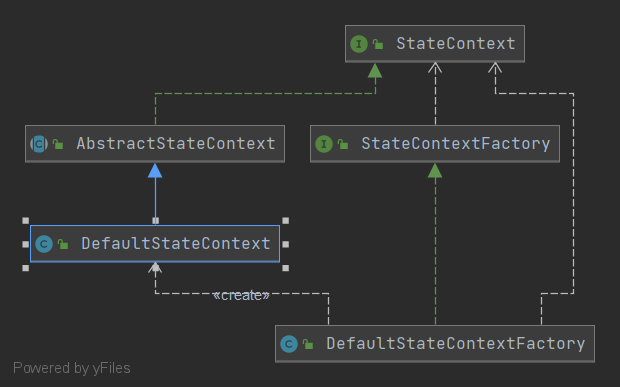
\includegraphics[width = 0.7 \textwidth]{images/class_diagrams/factory1.png}
    \caption{Class diagram of the Factory pattern instance recovered from \texttt{mina-statemachine}}
    \label{fig:factory1}
\end{figure}

\begin{figure}[H]
    \centering
    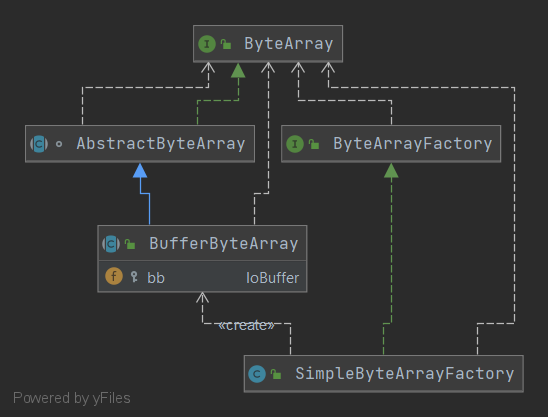
\includegraphics[width = 0.6 \textwidth]{images/class_diagrams/factory2.png}
    \caption{Class diagram of the Factory pattern instance recovered from \texttt{byteaccess}}
    \label{fig:factory2}
\end{figure}

\subsubsection{Removed patterns: Strategy pattern}
This section discusses the Strategy pattern within the scope of the \texttt{IoService} class. Pacito has recovered multiple instances of this pattern implemented in the \texttt{IoService} class throughout the analysed commit history; a variant of this pattern still exists in the current version of MINA. This shows that, despite its variations (which resulted in multiple pattern instances recovered), the Strategy pattern implemented in the \texttt{IoService} class can be considered a 'fundamental' pattern since it persisted until the current version of MINA. This also holds for other instances of the Strategy pattern found in similar scopes (e.g. \texttt{IoSession}). With the analysis of this Strategy pattern we aim at comparing its initial and final implementations, as well as investigating for revelatory clues of the changes that occurred in between.\\\\
\textsc{Pattern definition}: \textsc{Strategy} is a behavioural design pattern which allows for different class behaviours, which can be chosen at run time. Multiple strategy implementations are defined which extend the main strategy interface; a context object represents the context in which the strategy should be applied. Based on the chosen strategy implementation, the behaviour of the context object is subject to change \cite{strategy}\cite{strategy1}.\\\\
\textsc{Pattern implementation information from Pacito}:
\begin{itemize}
    \item \textsc{Initial instance}:
        \begin{itemize}
            \item \textsc{Strategy file}: \texttt{IoService}
            \item \textsc{Implementations}: 17 strategy implementations (see figure \ref{fig:strategy_removed})
            \item \textsc{Contexts}: \texttt{VmPipeSessionImpl}, \texttt{DatagramSessionImpl}, \texttt{SocketSessionImpl}
            \item \textsc{Delegator}: \texttt{IoService manager} in each of the contexts. 
        \end{itemize}
    \item \textsc{Current instance}:
        \begin{itemize}
            \item \textsc{Strategy file}: \texttt{IoService}
            \item \textsc{Implementations}: 7 strategy implementations (see figure \ref{fig:strategy_current})
            \item \textsc{Contexts}: \texttt{DefaultSocketSessionConfig}, \texttt{IoServiceStatistics}
            \item \textsc{Delegator}: \texttt{IoService parent}, \texttt{IoService service} 
        \end{itemize}
\end{itemize}
\textsc{Implementation \& class diagram}: The implementations of the strategy are captured by figures \ref{fig:strategy_removed} and \ref{fig:strategy_current}. The \texttt{IoService} is the backbone of any MINA based application (see section \ref{sec:analysis_components}); it needs to 'adapt' based on the type of network communication (i.e. TCP, UDP or in VM communication) and the participant to the communication (i.e. either a server, acceptor, or a client, connector). This idea is being concretized by the concept behind the Strategy pattern, where the \texttt{IoService} is the base strategy and the strategy implementations correspond with the above mentioned 'adaptations'. The strategies can be accessed through a \texttt{delegator}, a basic \texttt{IoService} object which expose the different implementations. In the initial Strategy pattern (see figure \ref{fig:strategy_removed}) a larger variety of implementations is present; in the latest version (see figure \ref{fig:strategy_current}), the number of strategy implementations has been reduced to a small number of essential interfaces which can further facilitate the user implementation of more specific strategies for their applications (e.g. \texttt{AbstractIoService} which stands as a base implementation for \texttt{IoService}); also, the in VM communication is not explicitly treated as a strategy. The contexts also differ between the initial and final version: the initial version employed the Strategy pattern in the context of defining base session implementations for each of the communication types, while in the final version, only one default or base implementation is presented (the level of generalization here is higher than in the initial version). Moreover, the final version introduces the \texttt{IoServiceStatistics} which corresponds to a more recent feature which provides statistics about number of connections, idle times etc.\\\\
\textsc{Issue tracking \&  motivation}: The motivation of introducing this pattern has been touched upon within the implementation discussion above. What is interesting to us, is the motivation behind the changes that occurred to this pattern throughout the commit history; we identify the following motivations based on the commit messages related to this pattern:
\begin{itemize}
    \item Resolving issues (mostly, JIRA listed) by improving the pattern or removing elements from it. For example:
        \begin{itemize}
            \item \textit{Resolved issue: DIRMINA-290 (Make IoService (IoConnector and IoAcceptor) manage only one service.)
* IoService (IoAcceptor and IoConnector) now can handler only one service at once.
** No more default settings.
* Merged IoServiceConfig implementations into the respective IoService implementations as setters.
* Removed a few spring framework integration classes which is not necessary now.(Binding and IoAcceptorBeanFactory)}
        \end{itemize}
    \item Updates or improvements to the code to fit the growth of the project as a whole. For example:
        \begin{itemize}
            \item \textit{* Added IoSessionConfig and its implementations
* Added IoServiceConfig and its implementations
* Added IoAcceptorConfig and its implementations
* Added IoConnectorConfig and its implementations
* Replaced all transport-type specific properties with the Config classes above}
        \end{itemize}
    \item Re-namings/refactorings or updates needed for integration or maintenance purposes. For example:
        \begin{itemize}
            \item \textit{* Renamed Base* to Abstract* which sounds more familiar to most developers
* Renamed DelegatedIoAcceptor to IoAcceptorWrapper and DelegatedIoConnector to IoConnectorWrapper respectively
* Renamed SessionIdleStatusChecked to IdleStatusChecker to make its name get aligned with IdleStatus type
* Renamed SessionLog to IoSessionLogger to make its name get aligned with IoSession type and SLF4J Logger type}
        \end{itemize}
\end{itemize}
Despite the alteration, the concept entailed by the Strategy pattern persisted within this scope, which means that the pattern was a good fit for the problem intended to solve. Discussion between developers regarding the implementation of this pattern is minimal, no concrete indicator towards the fact that they correlate having modeled multiple, behaviour changing variants of \texttt{IoService} to the Strategy pattern.\\\\
\textsc{Impact on architecture}: As it can be seen from figures \ref{fig:strategy_removed} and \ref{fig:strategy_current}, the number of classes required for the implementation of this pattern has reduced significantly from the introduction of the first instance. The current architecture reflects an emphasis on generalization and higher levels of abstraction. This is an indicator of how the project has matured over its development. \\\\
\textsc{Preliminary conclusions}: The chosen Strategy pattern instance seems to fit the context in which it has been introduced. Similar Strategy pattern approaches have also been taken for components that require the same 'adaptations' as the \texttt{IoService} one. However, it is difficult to establish if the introduction of the pattern has been explicitly debated by the developers: from the mailing lists and JIRA tickets, there are little to no explicit mentions of this pattern. It might be the case that the developer community is not fully or actively aware of the existence of this pattern or that the choice made towards this implementation (which coincides with the implementation of a Strategy pattern) was not necessarily pursued to implement said pattern.  


\begin{figure}
    \centering
    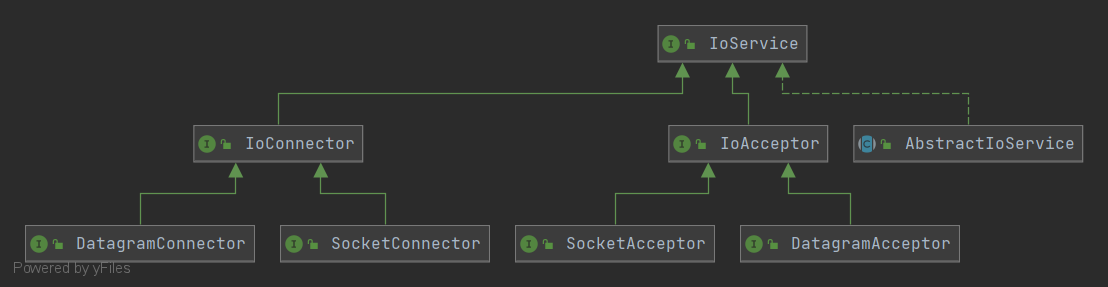
\includegraphics[width = \textwidth ]{images/class_diagrams/strategy_current.png}
    \caption{Class diagram of the the current Strategy pattern instance in \texttt{IoService}, capturing the strategy possible implementations; the context files are not shown in this diagram.}
    \label{fig:strategy_current}
\end{figure}


\begin{landscape}
    \begin{figure}
        \centering
        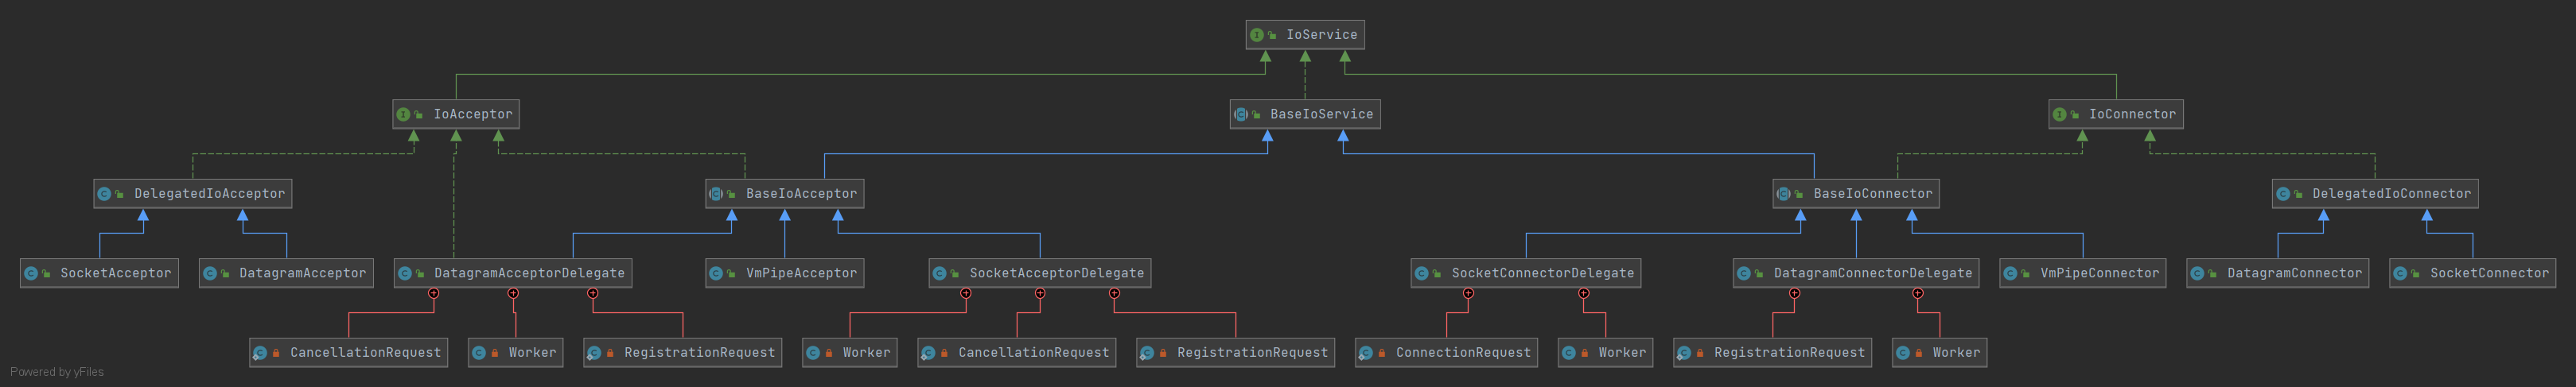
\includegraphics[scale = 0.2 ]{images/class_diagrams/strategy_removed.png}
        \caption{Class diagram of the initial (now removed) Strategy pattern instance in \texttt{IoService}, capturing the strategy possible implementations; the context files are not shown in this diagram.}
        \label{fig:strategy_removed}
    \end{figure}
\end{landscape}










\newpage
\addcontentsline{toc}{section}{References}
{
\setlength{\bibitemsep}{.7\baselineskip}
\printbibliography
}
\newpage

\begin{appendices}
\section{Figure excerpts from documentation sources}
\begin{figure}[H]
    \centering
    \begin{subfigure}[b]{0.5\textwidth}
         \centering
         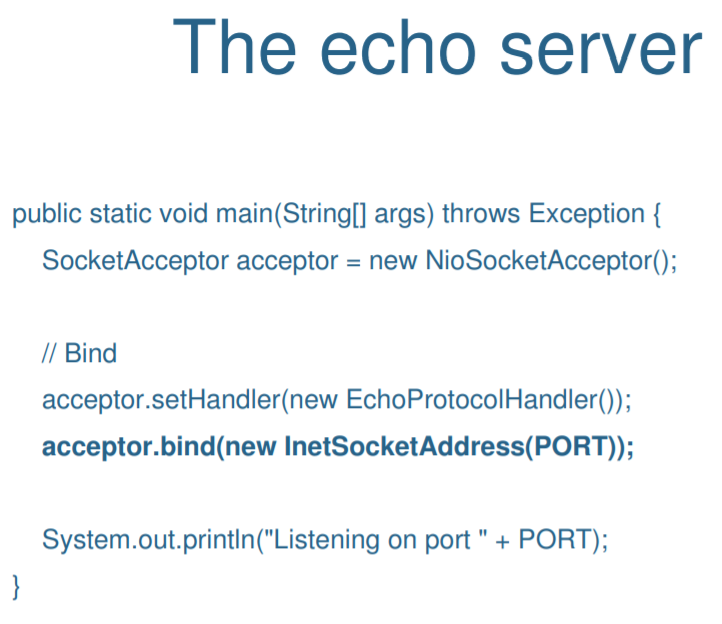
\includegraphics[width=\textwidth]{images/usability_extensibility1.png}
     \end{subfigure}
   
     \begin{subfigure}[b]{0.5\textwidth}
         \centering
         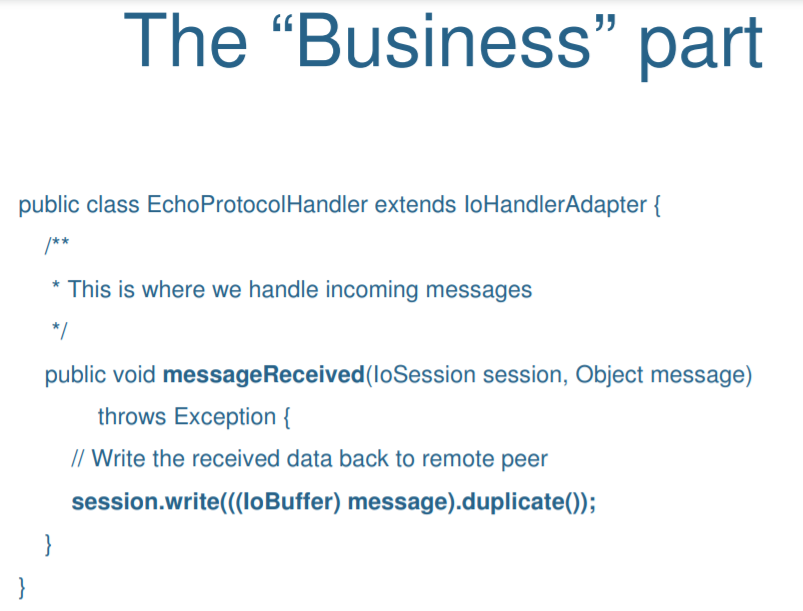
\includegraphics[width=\textwidth]{images/usability_extensibility2.png}
     \end{subfigure}
   
    \begin{subfigure}[b]{0.5\textwidth}
         \centering
         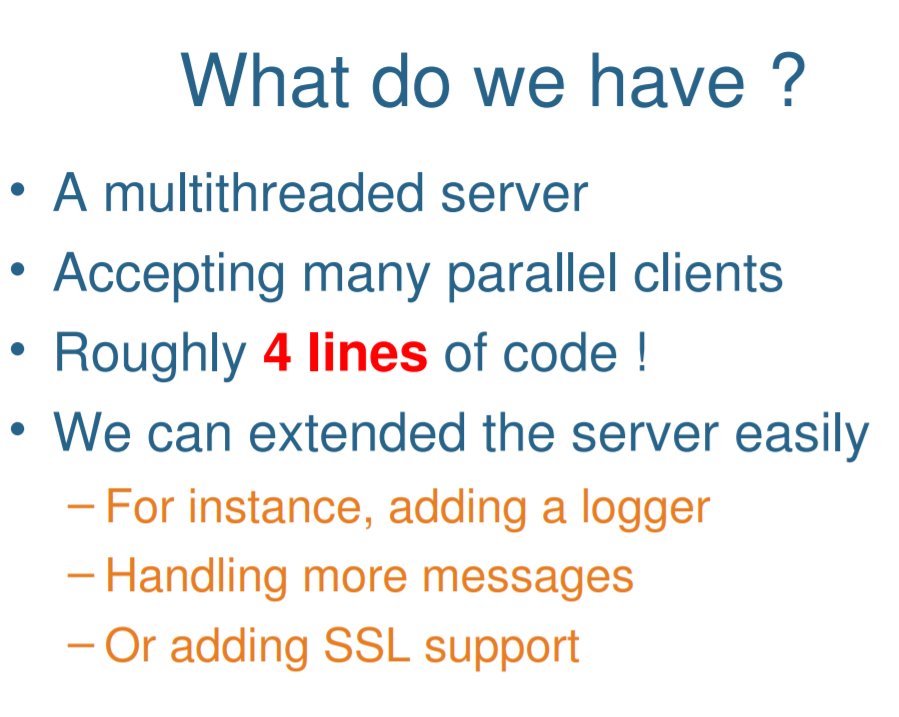
\includegraphics[width=\textwidth]{images/usability_extensibility.png}
     \end{subfigure}
    
    \caption{An exercept from \cite{mina-talk2009} that showcases the ease of use and extensibility of the MINA framework.}
    \label{fig:usability_extensibility}
\end{figure}

\begin{figure}[H]
    \centering
    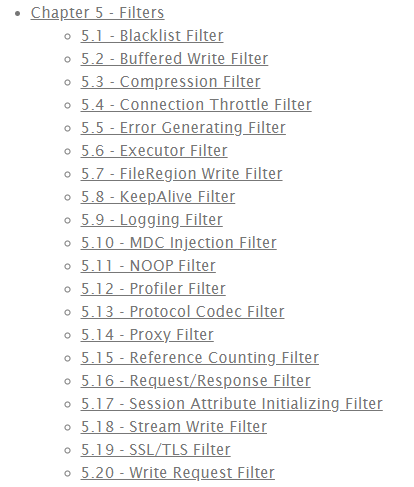
\includegraphics[width=0.6\textwidth]{images/filters.png}
    \caption{An overview of the out-of-the-box filters offered by the MINA framework; the overview has been extracted from \cite{mina-userguide}.}
    \label{fig:filters}
\end{figure}

\begin{figure}[H]
    \centering
    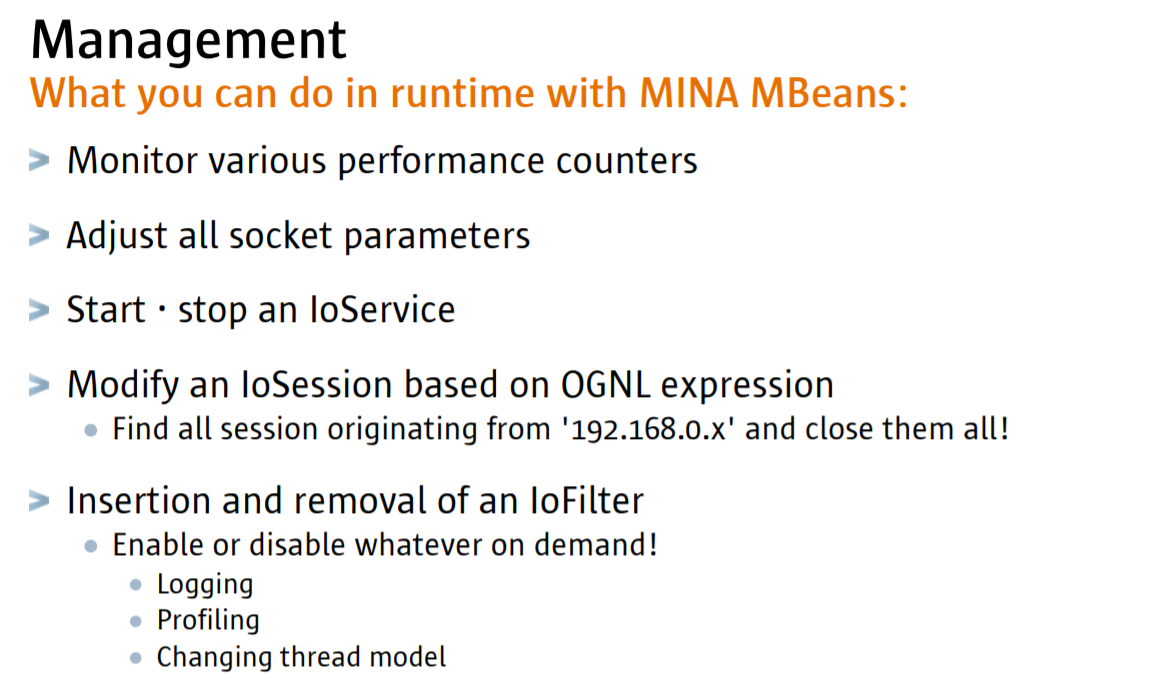
\includegraphics[width=0.7\textwidth]{images/management.png}
    \caption{Excerpt from \cite{mina-talk2008} showing the runtime management capabilities of MINA applications integrated with JMX.}
    \label{fig:manageability}
\end{figure}

\begin{figure}[H]
    \centering
    \begin{subfigure}[b]{0.7\textwidth}
         \centering
         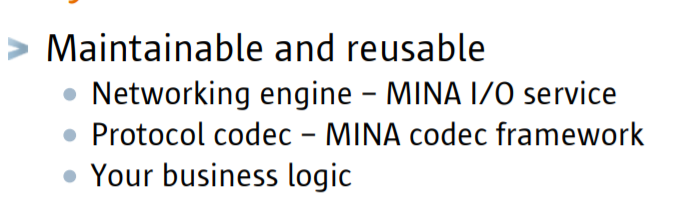
\includegraphics[width=\textwidth]{images/reusable1.png}
     \end{subfigure}

     \begin{subfigure}[b]{0.7\textwidth}
         \centering
         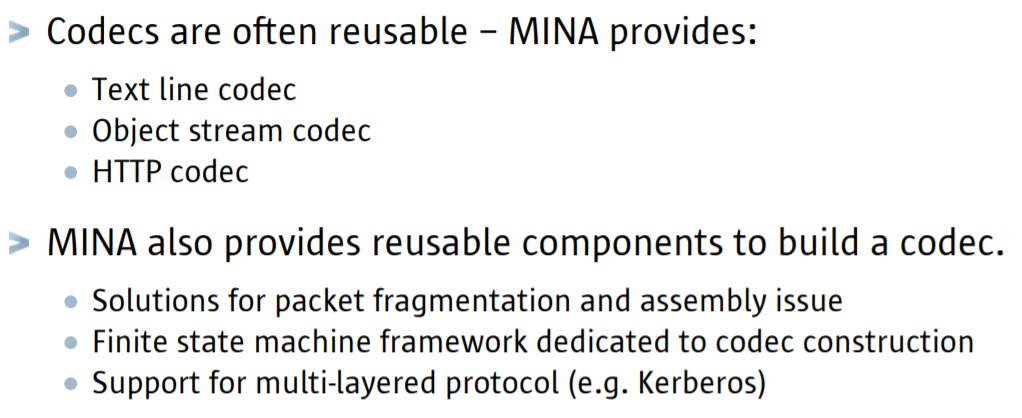
\includegraphics[width=\textwidth]{images/reusable.png}
     \end{subfigure}
     
    \begin{subfigure}[b]{0.7\textwidth}
         \centering
         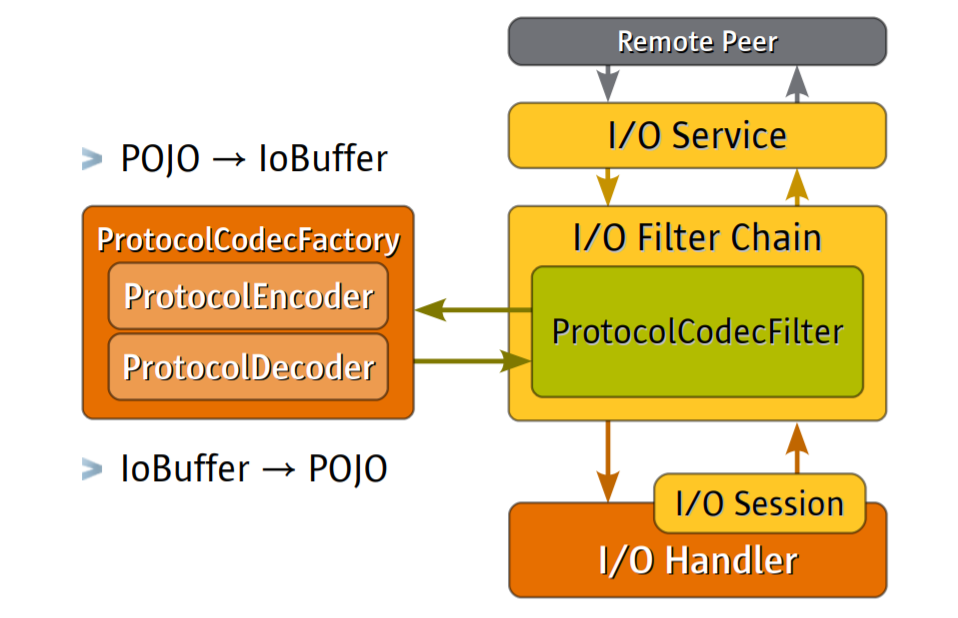
\includegraphics[width=\textwidth]{images/architecture_codec.png}
     \end{subfigure}
    
    \caption{An exercept from the presentation \cite{mina-talk2008} that showcases the high reusability  of components from the MINA framework.}
    \label{fig:reusability}
\end{figure}
\newpage
\section{Overview of the high-level architecture}

\begin{figure}[H]
    \centering
    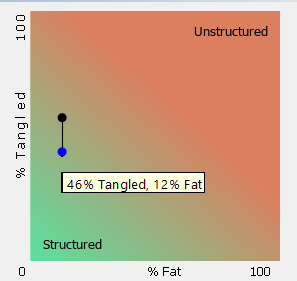
\includegraphics{images/tangles.png}
    \caption{Evolution of the 'tangle' and 'fat' metrics after the architectural restructuring of MINA, as extracted from the Structure101 project.}
    \label{fig:tangles}
\end{figure}

\begin{landscape}
\begin{figure}
    \centering
    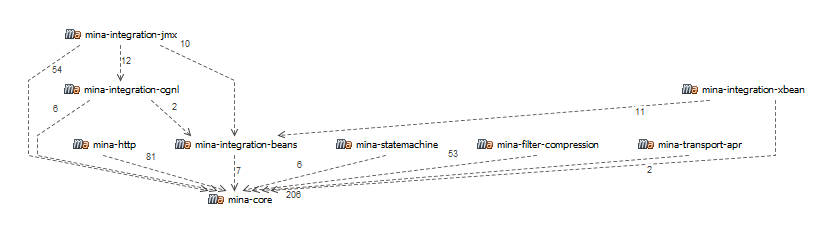
\includegraphics[scale=0.9]{images/MINA_package_dependencies.png}
    \caption{High-level overview of the MINA packages and their dependencies}
    \label{fig:overview_package_dependencies}
\end{figure}
\end{landscape}

\section{Overview of architectural components}
\subsection{MINA core}
\begin{figure}[H]
    \centering
    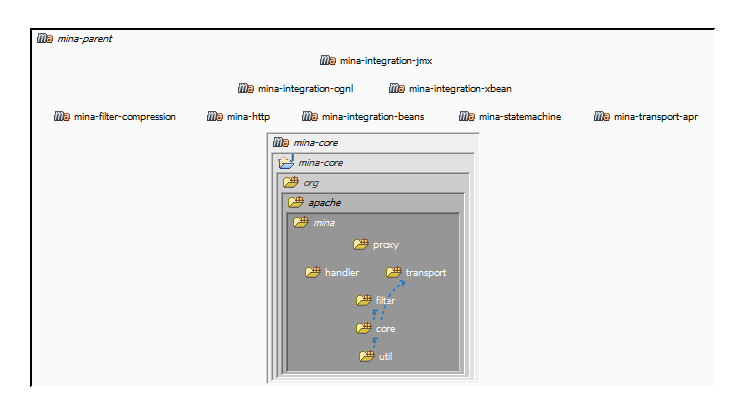
\includegraphics[width=\textwidth]{images/MINA_core_initial.png}
    \caption{Initial high-level structure of the \texttt{mina-core} module.}
    \label{fig:mina_core_initial}
\end{figure}

\begin{figure}[H]
    \centering
    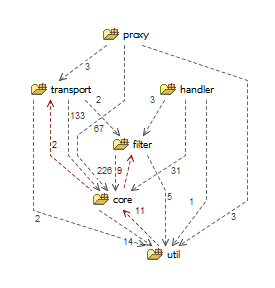
\includegraphics{images/MINA_core_initial_dependencies.png}
    \caption{Initial high-level dependency graph of the \texttt{mina-core} module}.
    \label{fig:mina_core_dependencies_initial}
\end{figure}

\begin{figure}[H]
    \centering
    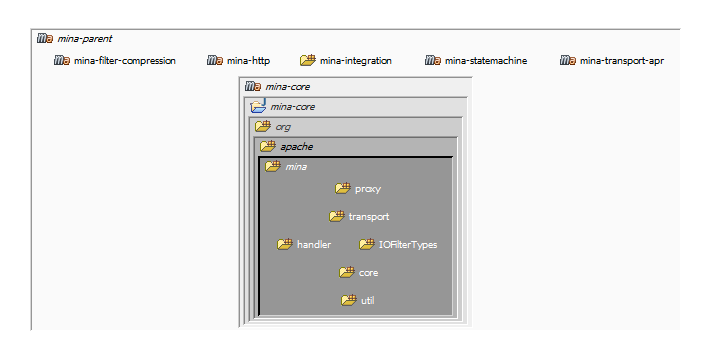
\includegraphics[width=\textwidth]{images/MINA_core_restructure.png}
    \caption{High-level structure of the \texttt{mina-core} module after restructuring.}
    \label{fig:mina_core_restructured}
\end{figure}

\begin{figure}[H]
    \centering
    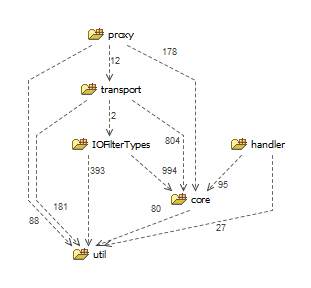
\includegraphics{images/MINA_core_dependencies_restructure.png}
    \caption{High-level dependency graph of the \texttt{mina-core} module after restructuring.}
    \label{fig:mina_core_dependencies_restructured}
\end{figure}

\begin{landscape}
\begin{figure}
    \centering
    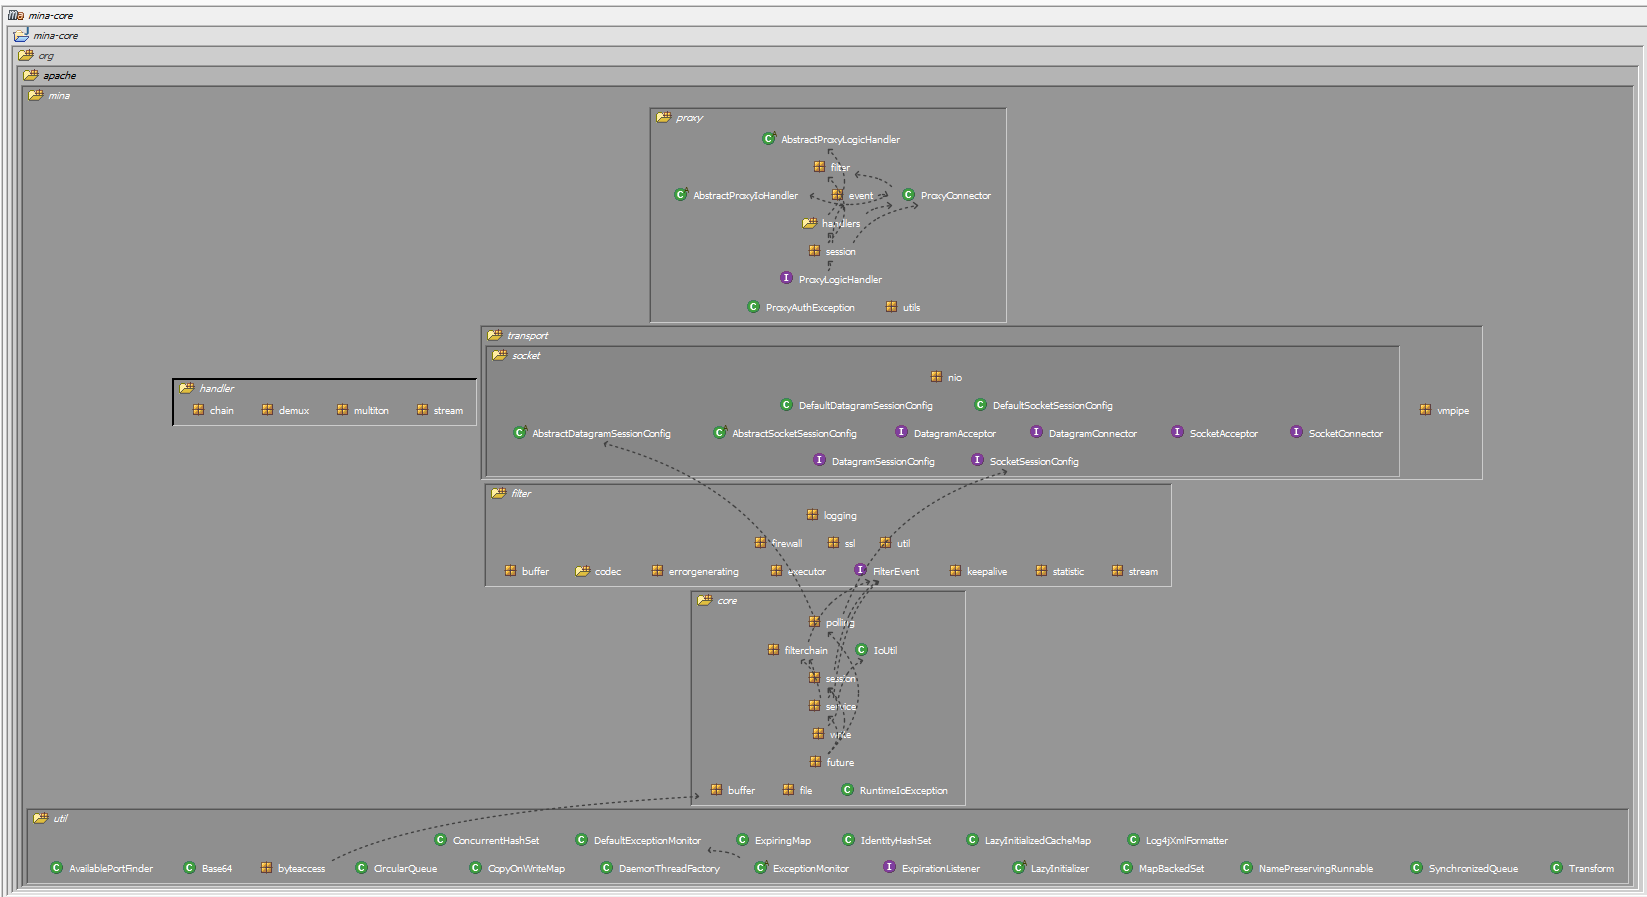
\includegraphics[width=\linewidth]{images/MINA_core_extended_initial.png}
    \caption{Detailed view of \texttt{mina-core} module.}
    \label{fig:mina_core_initial_detailed}
\end{figure}
\end{landscape}

\begin{landscape}
\begin{figure}
    \centering
    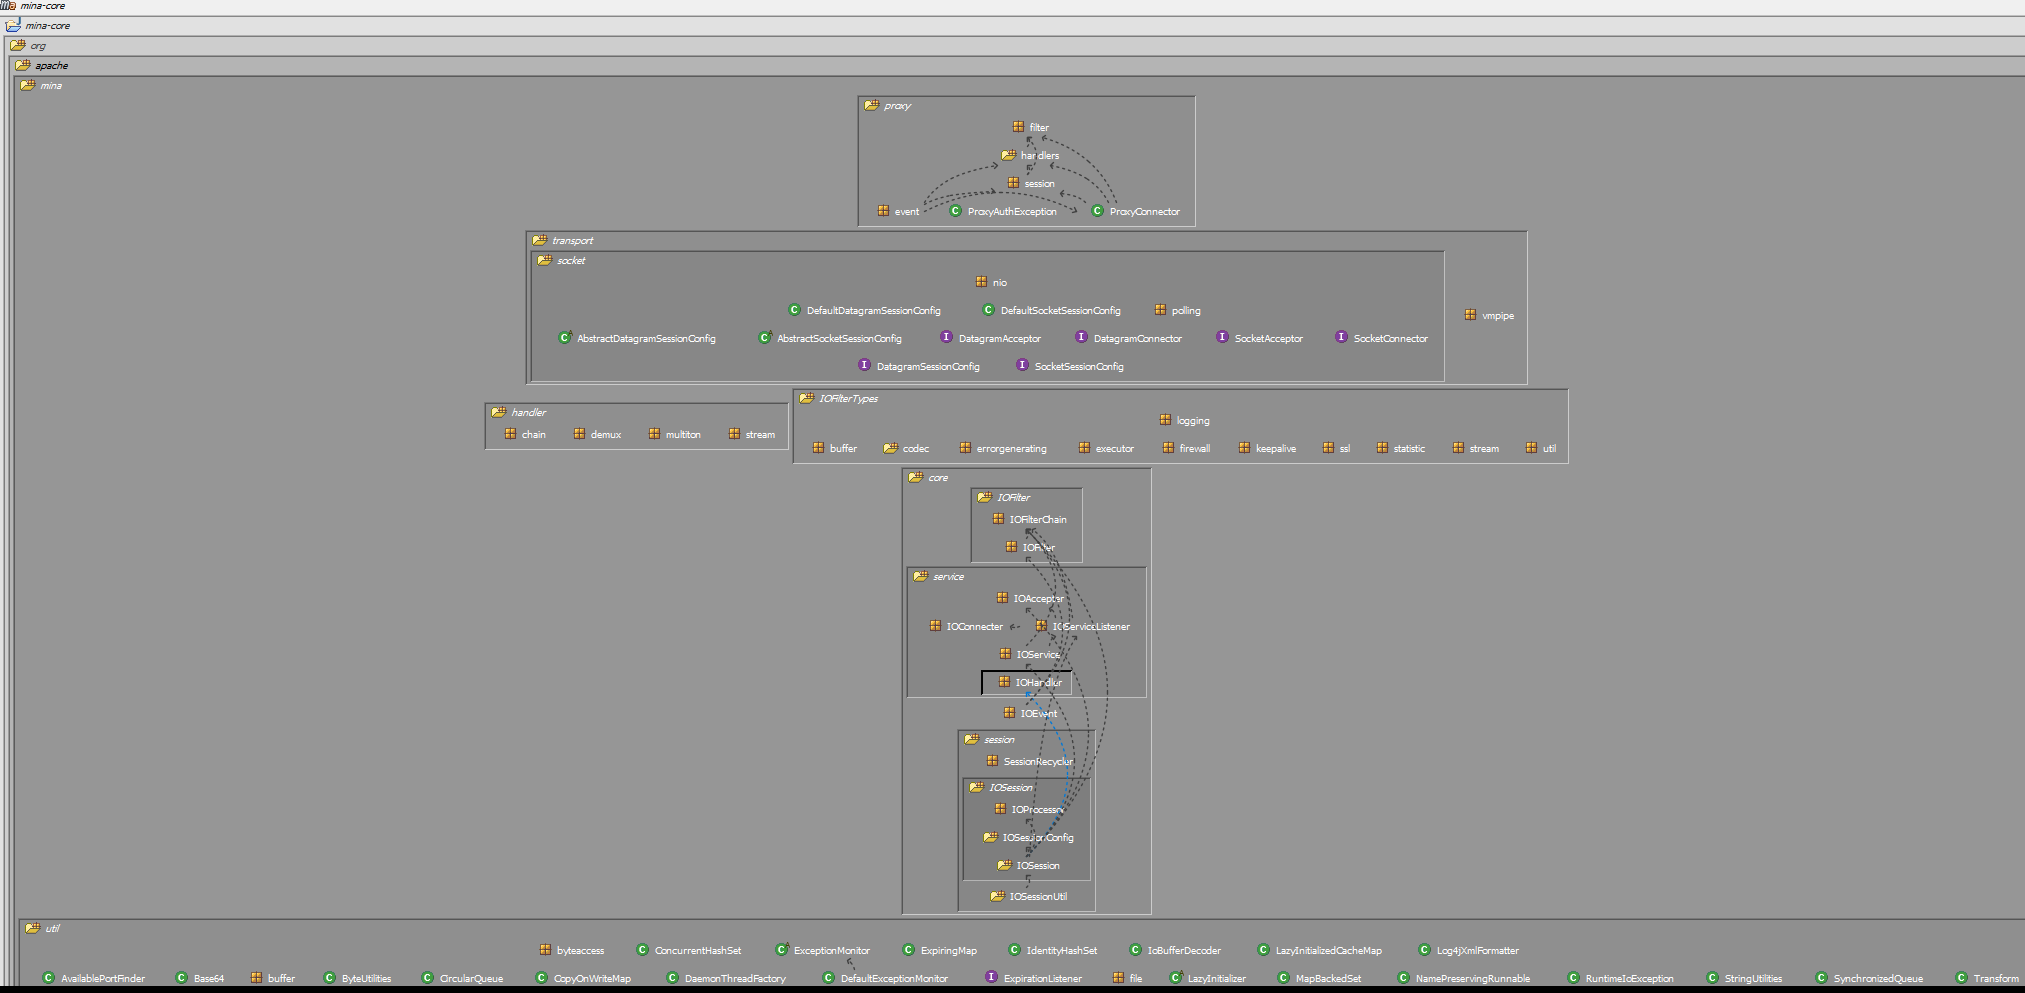
\includegraphics[scale=0.4]{images/MINA_core_extended_restructured.png}
    \caption{Detailed view of the restructured \texttt{mina-core} module.}
    \label{fig:mina_core_restructured_detailed}
\end{figure}
\end{landscape}

\subsubsection{MINA \texttt{core} component from the core module}

\begin{figure}[H]
    \centering
    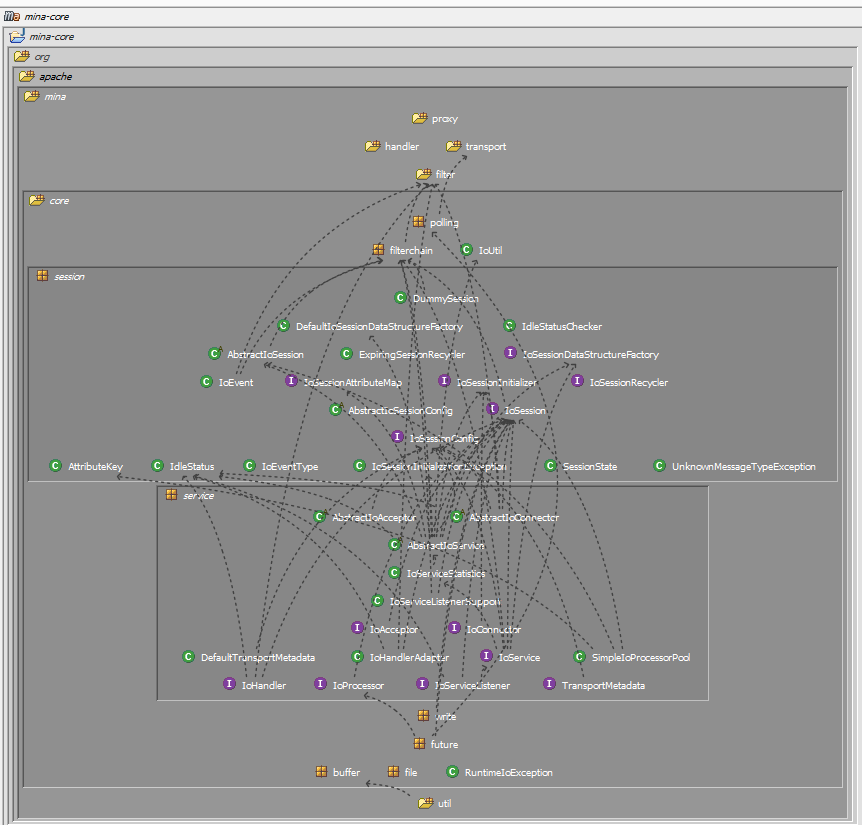
\includegraphics[scale = 0.7]{images/MINA_core_core_initial.png}
    \caption{Structure of the \texttt{mina-core-core} module.}
    \label{fig:mina_core_core_initial}
\end{figure}

\begin{figure}[H]
    \centering
    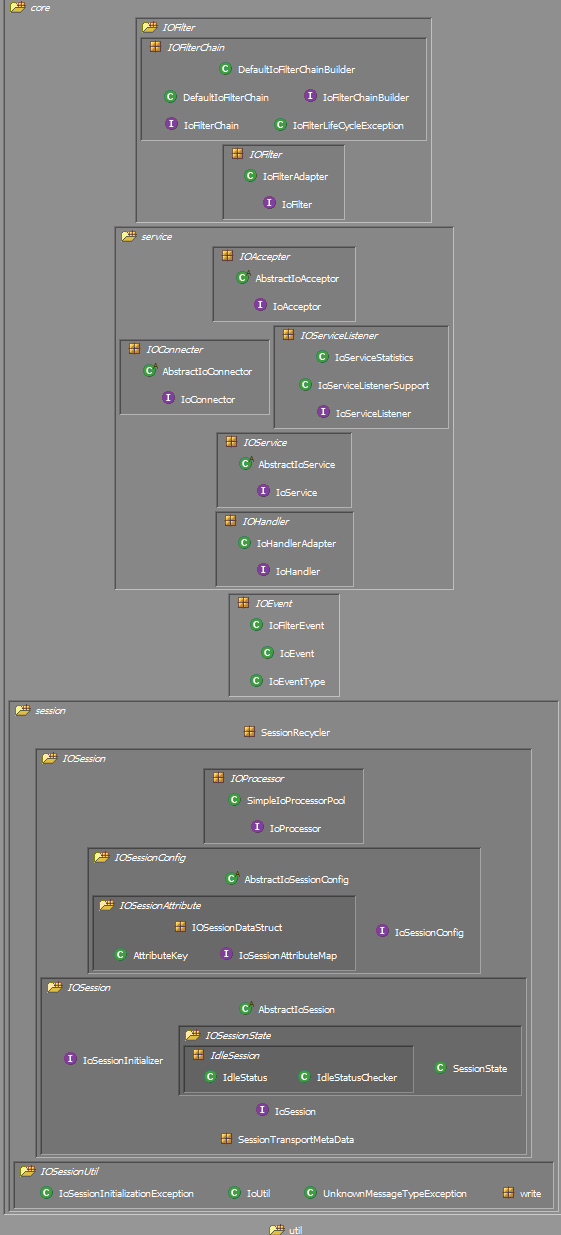
\includegraphics[scale=0.7]{images/MINA_core_core_restructured.png}
    \caption{Restructured \texttt{mina-core-core} module.}
    \label{fig:mina_core_core_restructured}
\end{figure}

\begin{figure}[H]
    \centering
    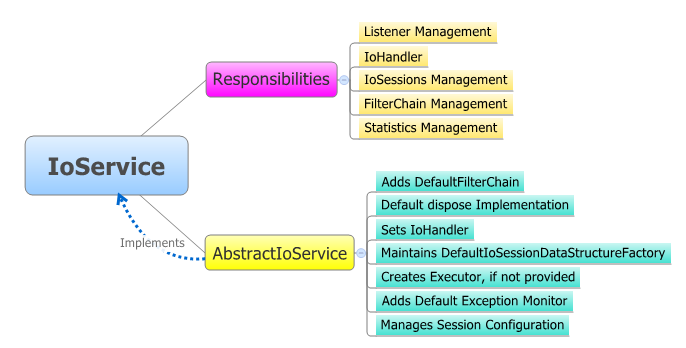
\includegraphics[width=\textwidth]{images/IoService_mindmap.png}
    \caption{Overview of the responsibilities of the \texttt{mina-core-core-service} component extracted from \cite{mina-userguide}.}
    \label{fig:service_responisbilities}
\end{figure}

\begin{figure}[H]
    \centering
    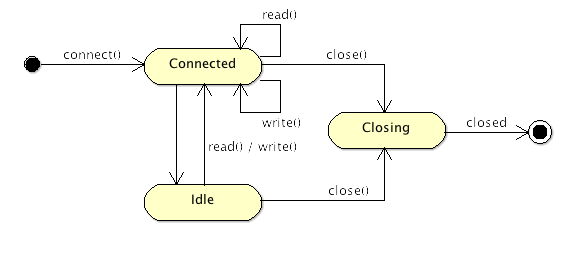
\includegraphics[width=\textwidth]{images/session-state.png}
    \caption{Visualisation of a session's life cycle, capturing the possible session states, extracted from \cite{mina-userguide}.}
    \label{fig:session_lifecycle}
\end{figure}


\subsection{MINA integration}

\begin{figure}[H]
    \centering
    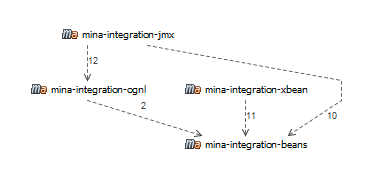
\includegraphics{images/MINA_integration_dependencies.png}
    \caption{MINA integration packages dependencies}
    \label{fig:dependencies_integration}
\end{figure}

\begin{figure}[H]
    \centering
    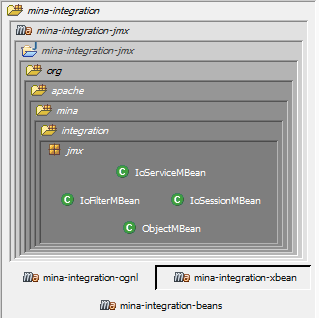
\includegraphics[width=0.5\textwidth]{images/MINA_integration_jmx.png}
    \caption{MINA JMX integration package}
    \label{fig:jmx_integration}
\end{figure}

\begin{figure}[H]
    \centering
    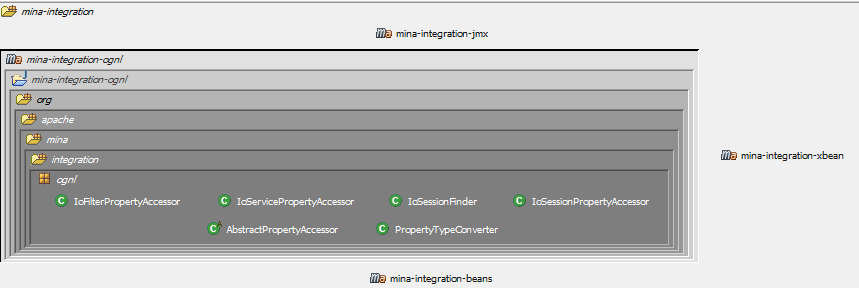
\includegraphics[width=\textwidth]{images/MINA_integration_ognl.png}
    \caption{MINA OGNL integration package}
    \label{fig:ognl_integration}
\end{figure}

\begin{figure}[H]
    \centering
    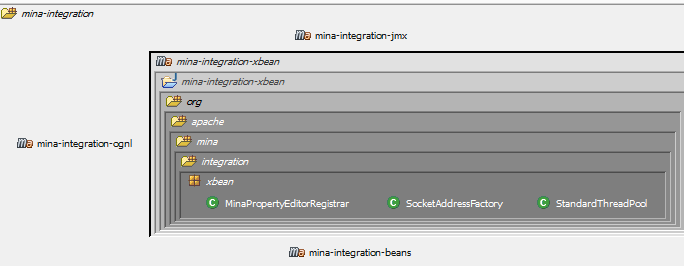
\includegraphics[width=\textwidth]{images/MINA_integration_xbean.png}
    \caption{MINA XBean integration package}
    \label{fig:xbean_integration}
\end{figure}

\begin{landscape}
\begin{figure}
    \centering
    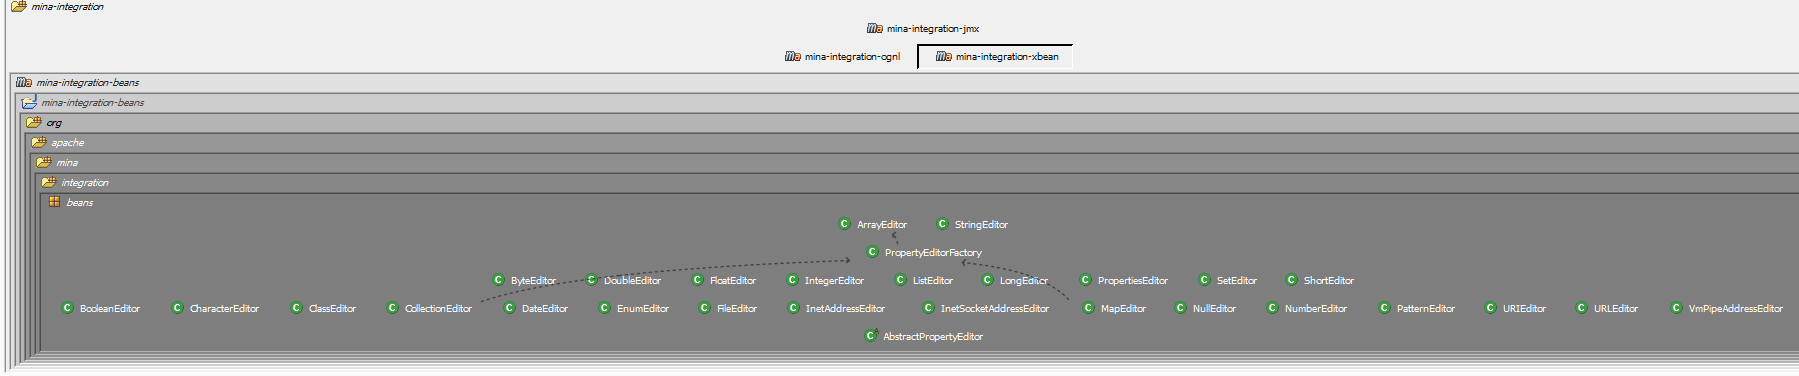
\includegraphics[scale=0.5]{images/MINA_integration_beans.png}
    \caption{MINA Beans integration package}
    \label{fig:beans_integration}
\end{figure}
\end{landscape}

\subsection{MINA state machine}

\begin{figure}[H]
    \centering
    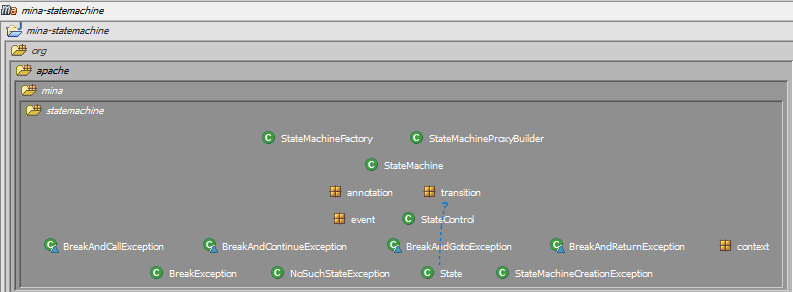
\includegraphics[width=\textwidth]{images/MINA_structure_statemachine_initial.png}
    \caption{Structure of the \texttt{statemachine} package}
    \label{fig:statemachine_initial}
\end{figure}

\begin{figure}[H]
    \centering
    \includegraphics[width=0.7\textwidth]{images/MINA_structure_statemachine_restructured.png}
    \caption{Overview of the \texttt{statemachine} package after restructuring}
    \label{fig:statemachine_restructured}
\end{figure}

\begin{landscape}
\begin{figure}
    \centering
    \includegraphics[scale = 0.5]{images/MINA_dependencies_statemachine_initial.png}
    \caption{Inner dependencies of the \texttt{statemachine} package}
    \label{fig:statemachine_initial_dependencies}
\end{figure}
\end{landscape}

\begin{figure}[H]
    \centering
    \includegraphics[scale = 0.8]{images/MINA_dependencies_statemachine_restructured.png}
    \caption{Inner dependencies of the \texttt{statemachine} package after restructuring}
    \label{fig:statemachine_restructured_dependencies}
\end{figure}

\begin{figure}[H]
    \centering
    \includegraphics[width=\textwidth]{images/state-diagram.png}
    \caption{A simple example of a state application which can be implemented using the state machine functionality of MINA; the example has been extracted from \cite{mina-userguide}.}
    \label{fig:statemachine_example}
\end{figure}

\subsection{MINA HTTP}

\begin{figure}[H]
    \centering
    \includegraphics[width=\textwidth]{images/MINA_http_structure_initial.png}
    \caption{Structure of the \texttt{http} package}
    \label{fig:http_structure_initial}
\end{figure}

\begin{figure}[H]
    \centering
    \includegraphics[width=\textwidth]{images/MINA_http_dependencies_initial.png}
    \caption{Inner dependencies of the \texttt{http} package}
    \label{fig:http_dependencies_initial}
\end{figure}

\begin{figure}[H]
    \centering
    \includegraphics{images/MINA_http_structure.png}
    \caption{Overview of the restructured \texttt{http} package}
    \label{fig:http_structure_restructured}
\end{figure}

\begin{figure}[H]
    \centering
    \includegraphics{images/MINA_http_dependencies.png}
    \caption{Inner dependencies of the restructured \texttt{http} package}
    \label{fig:http_dependencies_restructured}
\end{figure}

\subsection{MINA transport APR}

\begin{figure}[H]
    \centering
    \includegraphics{images/MINA_apr_structure.png}
    \caption{Structure of the \texttt{transport-apr} package}
    \label{fig:apr_structure}
\end{figure}

\begin{figure}[H]
    \centering
    \includegraphics[width=\textwidth]{images/MINA_apr_dependencies.png}
    \caption{Inner dependencies of the \texttt{transport-apr} package}
    \label{fig:apr_dependencies}
\end{figure}

\section{Call graphs for methods included in the create server use case}
\label{sec:call_graphs}

\begin{figure}[H]
    \centering
    \includegraphics[width=\textwidth]{images/getfilterchain.png}
    \caption{\texttt{getFilterChain} call graph}
    \label{fig:getfilterchain}
\end{figure}
\begin{figure}[H]
    \centering
    \includegraphics[width=\textwidth]{images/buildfilterchain.png}
    \caption{\texttt{buildFilterChain} call graph}
    \label{fig:buildfilterchain}
\end{figure}

\begin{figure}[H]
    \centering
    \includegraphics{images/addlast.png}
    \caption{\texttt{addLast} call graph}
    \label{fig:addlast}
\end{figure}

\begin{figure}[H]
    \centering
    \includegraphics[width=\textwidth]{images/sethandler.png}
    \caption{\texttt{setHandler} call graph}
    \label{fig:sethandler}
\end{figure}

\begin{figure}[H]
    \centering
    \includegraphics[width=\textwidth]{images/getsessionconfig.png}
    \caption{\texttt{getSessionConfig} call graph}
    \label{fig:getSessionConfig}
\end{figure}


\begin{figure}[H]
    \centering
    \includegraphics[width=\textwidth]{images/setreadbuffersize.png}
    \caption{\texttt{setReadBufferSize} call graph}
    \label{fig:setreadbuffersize}
\end{figure}

\begin{figure}[H]
    \centering
    \includegraphics[width=\textwidth]{images/setidletime.png}
    \caption{\texttt{setIdleTime} call graph}
    \label{fig:setidletime}
\end{figure}










\newpage
\section{Changelog}

The following students have contributed to the elaboration of this document:
\begin{enumerate}
     \item Alina Matei s3080722 (ID: AM)
    \item Floris Westerman (ID: FW)
\end{enumerate}
   
\begin{table}[H]
    \centering
    \begin{tabular}{c|c|c}
        ID & Date & Task  \\
        \hline \hline
        \multicolumn{3}{c}{Week 1 (18/11/2020 - 25/11/2020)}\\
        \hline
        \multicolumn{3}{c}{Week 2(25/11/2020 - 02/12/2020)}\\
        \hline
        AM & 26/11/2020 & Implemented TA feedback 
    \end{tabular}
    \caption{Changelog table}
    \label{tab:changelog}
\end{table}
\end{appendices}

\end{document}
